\documentclass[a4paper,titlepage]{scrartcl}
\usepackage[francais]{babel}
\usepackage[T1]{fontenc}
\usepackage[utf8]{inputenc}

\usepackage{graphicx}
\usepackage{float} % Ncessaire pour les tables et figures dans l'environnement double colonne 


\usepackage{layout}

\usepackage{fancyhdr} % en-ttes et pieds de page 

\usepackage{hyperref} % hyperliens 

\usepackage{dtklogos}

% En-ttes et pieds de page 
\pagestyle{fancy}  
\fancyhead{} % Blank out the default header
\fancyfoot{} % Blank out the default footer
\fancyhead[C]{Rapport TX \no 4911 - Plateforme de voeux pour le suivi des stages GSM.} % Custom header text
\fancyfoot[R]{\thepage} % Custom footer text

% Disable header and footer rules
\setlength{\textheight}{650pt}

\newsavebox{\abstractbox}
\renewenvironment{abstract}
  {\begin{lrbox}{0}\begin{minipage}{\textwidth}
   \begin{center}\normalfont\sectfont\abstractname\end{center}\quotation}
  {\endquotation\end{minipage}\end{lrbox}%
   \global\setbox\abstractbox=\box0 }

\usepackage{etoolbox}
\makeatletter
\expandafter\patchcmd\csname\string\maketitle\endcsname
  {\vskip\z@\@plus3fill}
  {\vskip\z@\@plus2fill\box\abstractbox\vskip\z@\@plus1fill}
  {}{}
\makeatother

\usepackage{lipsum}

\begin{document}

%---------------------------------------------------------------------------------

\titlehead{Université de Technologie de Compiègne}
\title{Plateforme de voeux pour le suivi des stages GSM.\vspace{1cm}}
\subject{- Rapport TX \no 4911 -}
\author{Jonathan DEKHTIAR\\ \vspace{1cm}\\\textbf{- Suiveur TX -}\\Alexandre DURUPT – Département GSM\\MCF PG1/I105, Responsable stages GSM\vspace{1cm}}

\renewcommand{\abstractname}{Sujet de la TX}
\begin{abstract}

L'objectif de cette TX est de revoir la démarche d'attribution des suiveurs UTC dans le cadre des stages TN09 et TN10 du GSM. A ce jour l'attribution est réalisée manuellement et ne tient pas compte réellement des voeux exprimés par les personnels. La mission de la TX sera, à partir d'une feuille Excel regroupant la liste des stages (titre, lieu, etc.), de créer une interface VBA ou html permettant prise en compte des voeux et leur ordonnancement. Cette interface pourra également permettre l'export au format Excel des résultats.
\end{abstract}

\maketitle


%----------------------------------------------------------------------------------------

\tableofcontents
\clearpage

%------------------------------------------------------------------------------


\section{Le cahier des charges}


\subsection{Objectifs de la TX}

Réalisation d’un frontend/backend online sur l’intranet de l’UTC qui permettra l’automatisation du processus de réalisation des voeux d’attribution des stages TN09/TN10 pour les suiveurs de stage du département GSM.

\subsection{Les Contraintes}

\begin{itemize}
	\item L’outil devra être capable de réaliser un export final au format Excel afin de pouvoir procéder à l’attribution des voeux. Format identique à celui utilisé actuellement.\\
	
	\item L’outil devra être capable de réaliser un import automatique des données par upload d’un fichier Excel pour chaque catégorie de Stage : TN09 \& TN10.\\
	
	\item L’outil devra se baser sur des technologies webs compatibles avec l’architecture UTC (PHP / HTML / Javascript / MySQL).\\
	
	\item L’outil devra être commenté et disposé d’une documentation technique afin de permettre son support et sa mise à jour si nécessaire.\\
	
	\item L’outil devra permettre une notation de 0 (je n’en veux pas) à 5 (je le veux absolument). Ces notes doivent être visibles sur le fichier d’export.\\
	
	\item Il serait également souhaitable que l'on puisse visualiser l'ordre des votes (qui a voté en premier) dans le fichier d'export.\\
	
	\item La plateforme devra être administrable et manipulable par un \textbf{non-informaticien}.\\
	
	\item Les maitres mots du projet doivent être : \textbf{ergonomie, simplicité, intuitivité, rapidité.} \\
	
	\item La plateforme doit être sécurisée et hébergée sur les serveurs UTC pour des raisons de confidentialité. Si possible, l'utilisation du \textbf{CAS UTC} serait un réel avantage. \\
	
\end{itemize}

\vspace{1cm}

\Large
\begin{center}
\textbf{
- Adresse de la plateforme -\\
\url{https://affectation-suiveurs.gsm.utc.fr/}\\
}

\vspace{1cm}

\textbf{
- Adresse du projet GitHub -\\
\url{https://github.com/JonathanDekhtiar/TxChoixDesStages}\\
}
\end{center}
\normalsize

\clearpage

%------------------------------------------------------------------------------

\section{Le planning prévisionnel - Gantt}

\begin{figure}[H]
	\vspace{-3mm}
	\begin{center}
		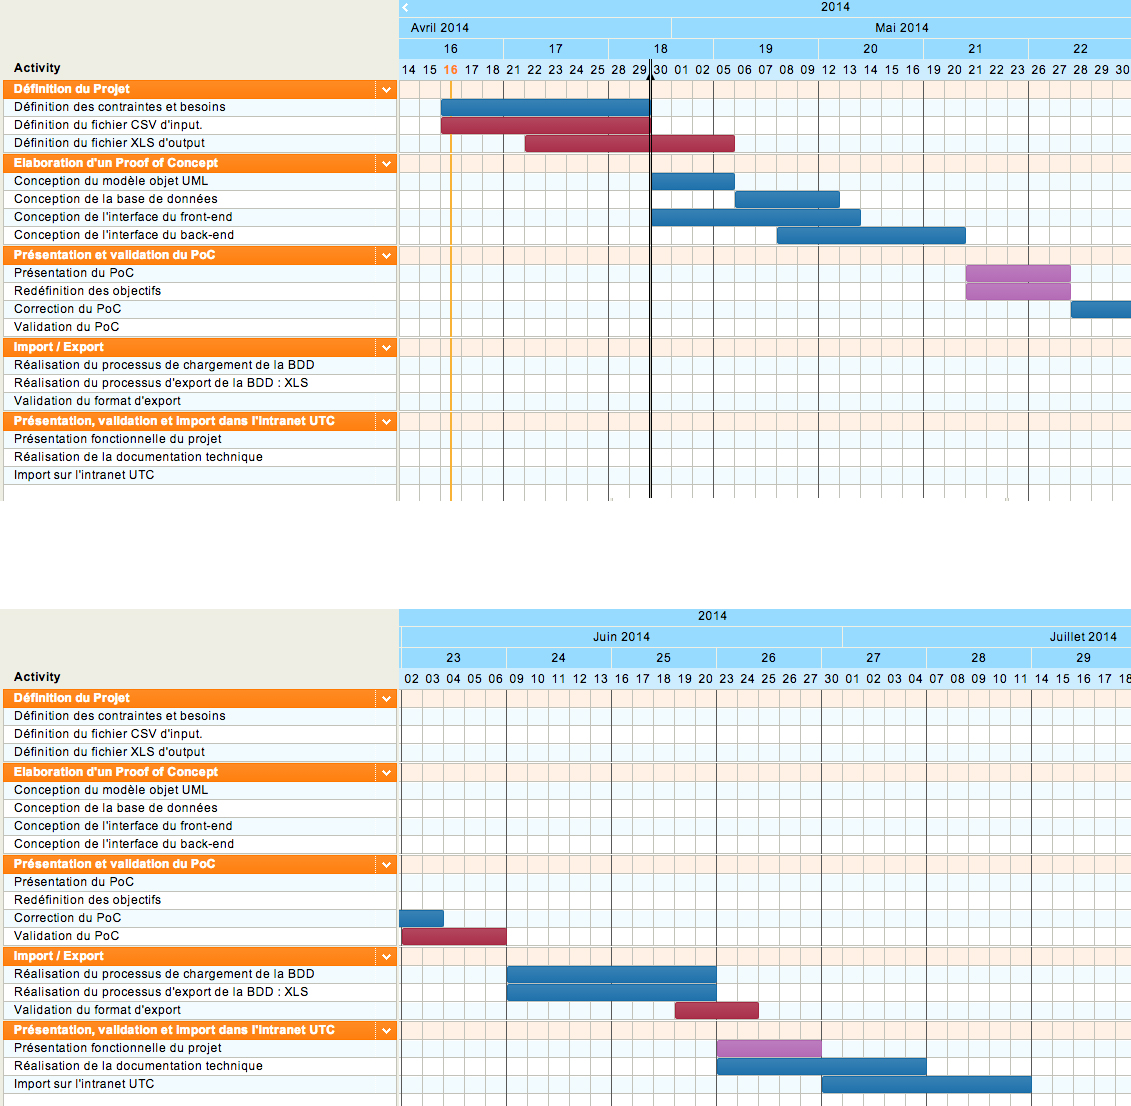
\includegraphics[scale=0.37]{Images/gantt.jpg}
		\caption{Diagramme de Gantt}
	\end{center}
\end{figure}

\clearpage

%------------------------------------------------------------------------------

\section{Utilisation de la plateforme - Point de vue Utilisateur}

\subsection{La page d'accueil}

\begin{figure}[H]
	\vspace{-3mm}
	\begin{center}
		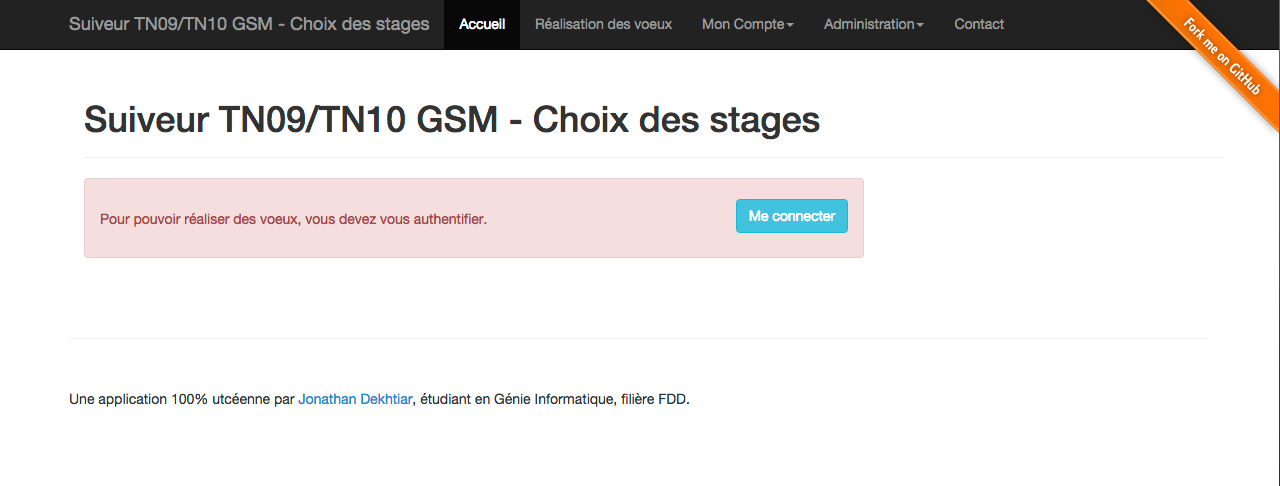
\includegraphics[scale=0.34]{Images/homepage_disconnected.png}
		\caption{La page d'accueil - Hors connexion}
	\end{center}
\end{figure}

Le site internet se trouve à l'adresse: \url{https://affectation-suiveurs.gsm.utc.fr/}.\\
Ce dernier est uniquement accessible que si l'utilisateur se trouve à l'intérieur du réseau UTC, soit en étant physiquement présent à l'UTC soit en utilisant le VPN.\\

Lors de son arrivé sur la plateforme, le site internet demande une identification, sans quoi rien n'est possible (excepté contacter les administrateurs).\\

En cliquant sur \textbf{Me Connecter}, l'utilisateur est redirigé vers le CAS UTC :\\

\begin{figure}[H]
	\vspace{-3mm}
	\begin{center}
		
\includegraphics[scale=0.34]{Images/casUTC.png}
		\caption{Page de Connexion - CAS UTC}
	\end{center}
	\vspace{-2cm}
\end{figure}

\clearpage

Une fois la connection effectuée, le site nous informe que nous sommes bien connecté.\\

\begin{figure}[H]
	\vspace{-3mm}
	\begin{center}
		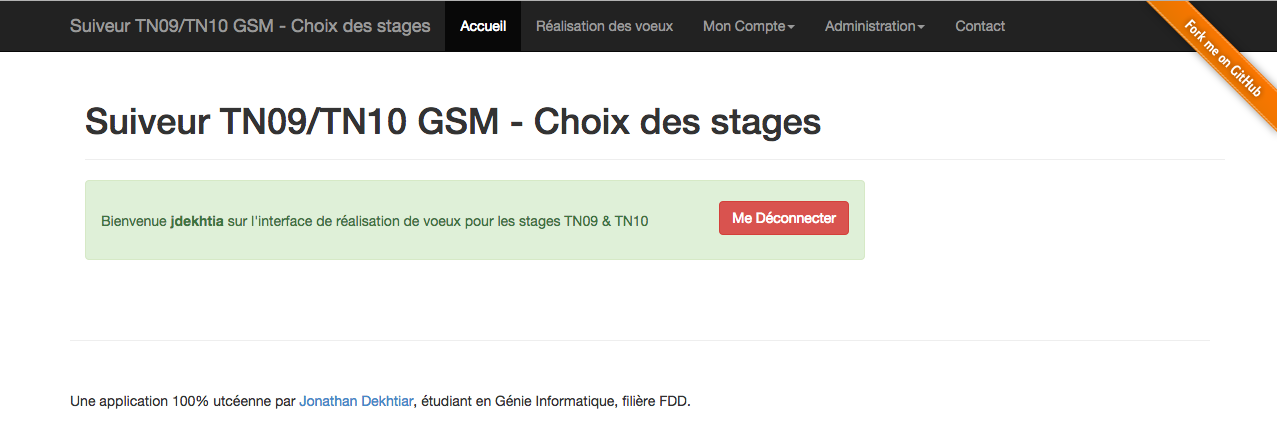
\includegraphics[scale=0.32]{Images/homepage_connected.png}
		\caption{La page d'accueil - Connexion Réussie}
	\end{center}
\end{figure}

\vspace{1cm}
\subsection{Renseigner ses informations personnelles}

Lors de la première connexion, le site internet vous demanderas de renseigner vos informations personnelles : \textbf{Nom / Prénom / Email}.\\

\begin{figure}[H]
	\vspace{-3mm}
	\begin{center}
		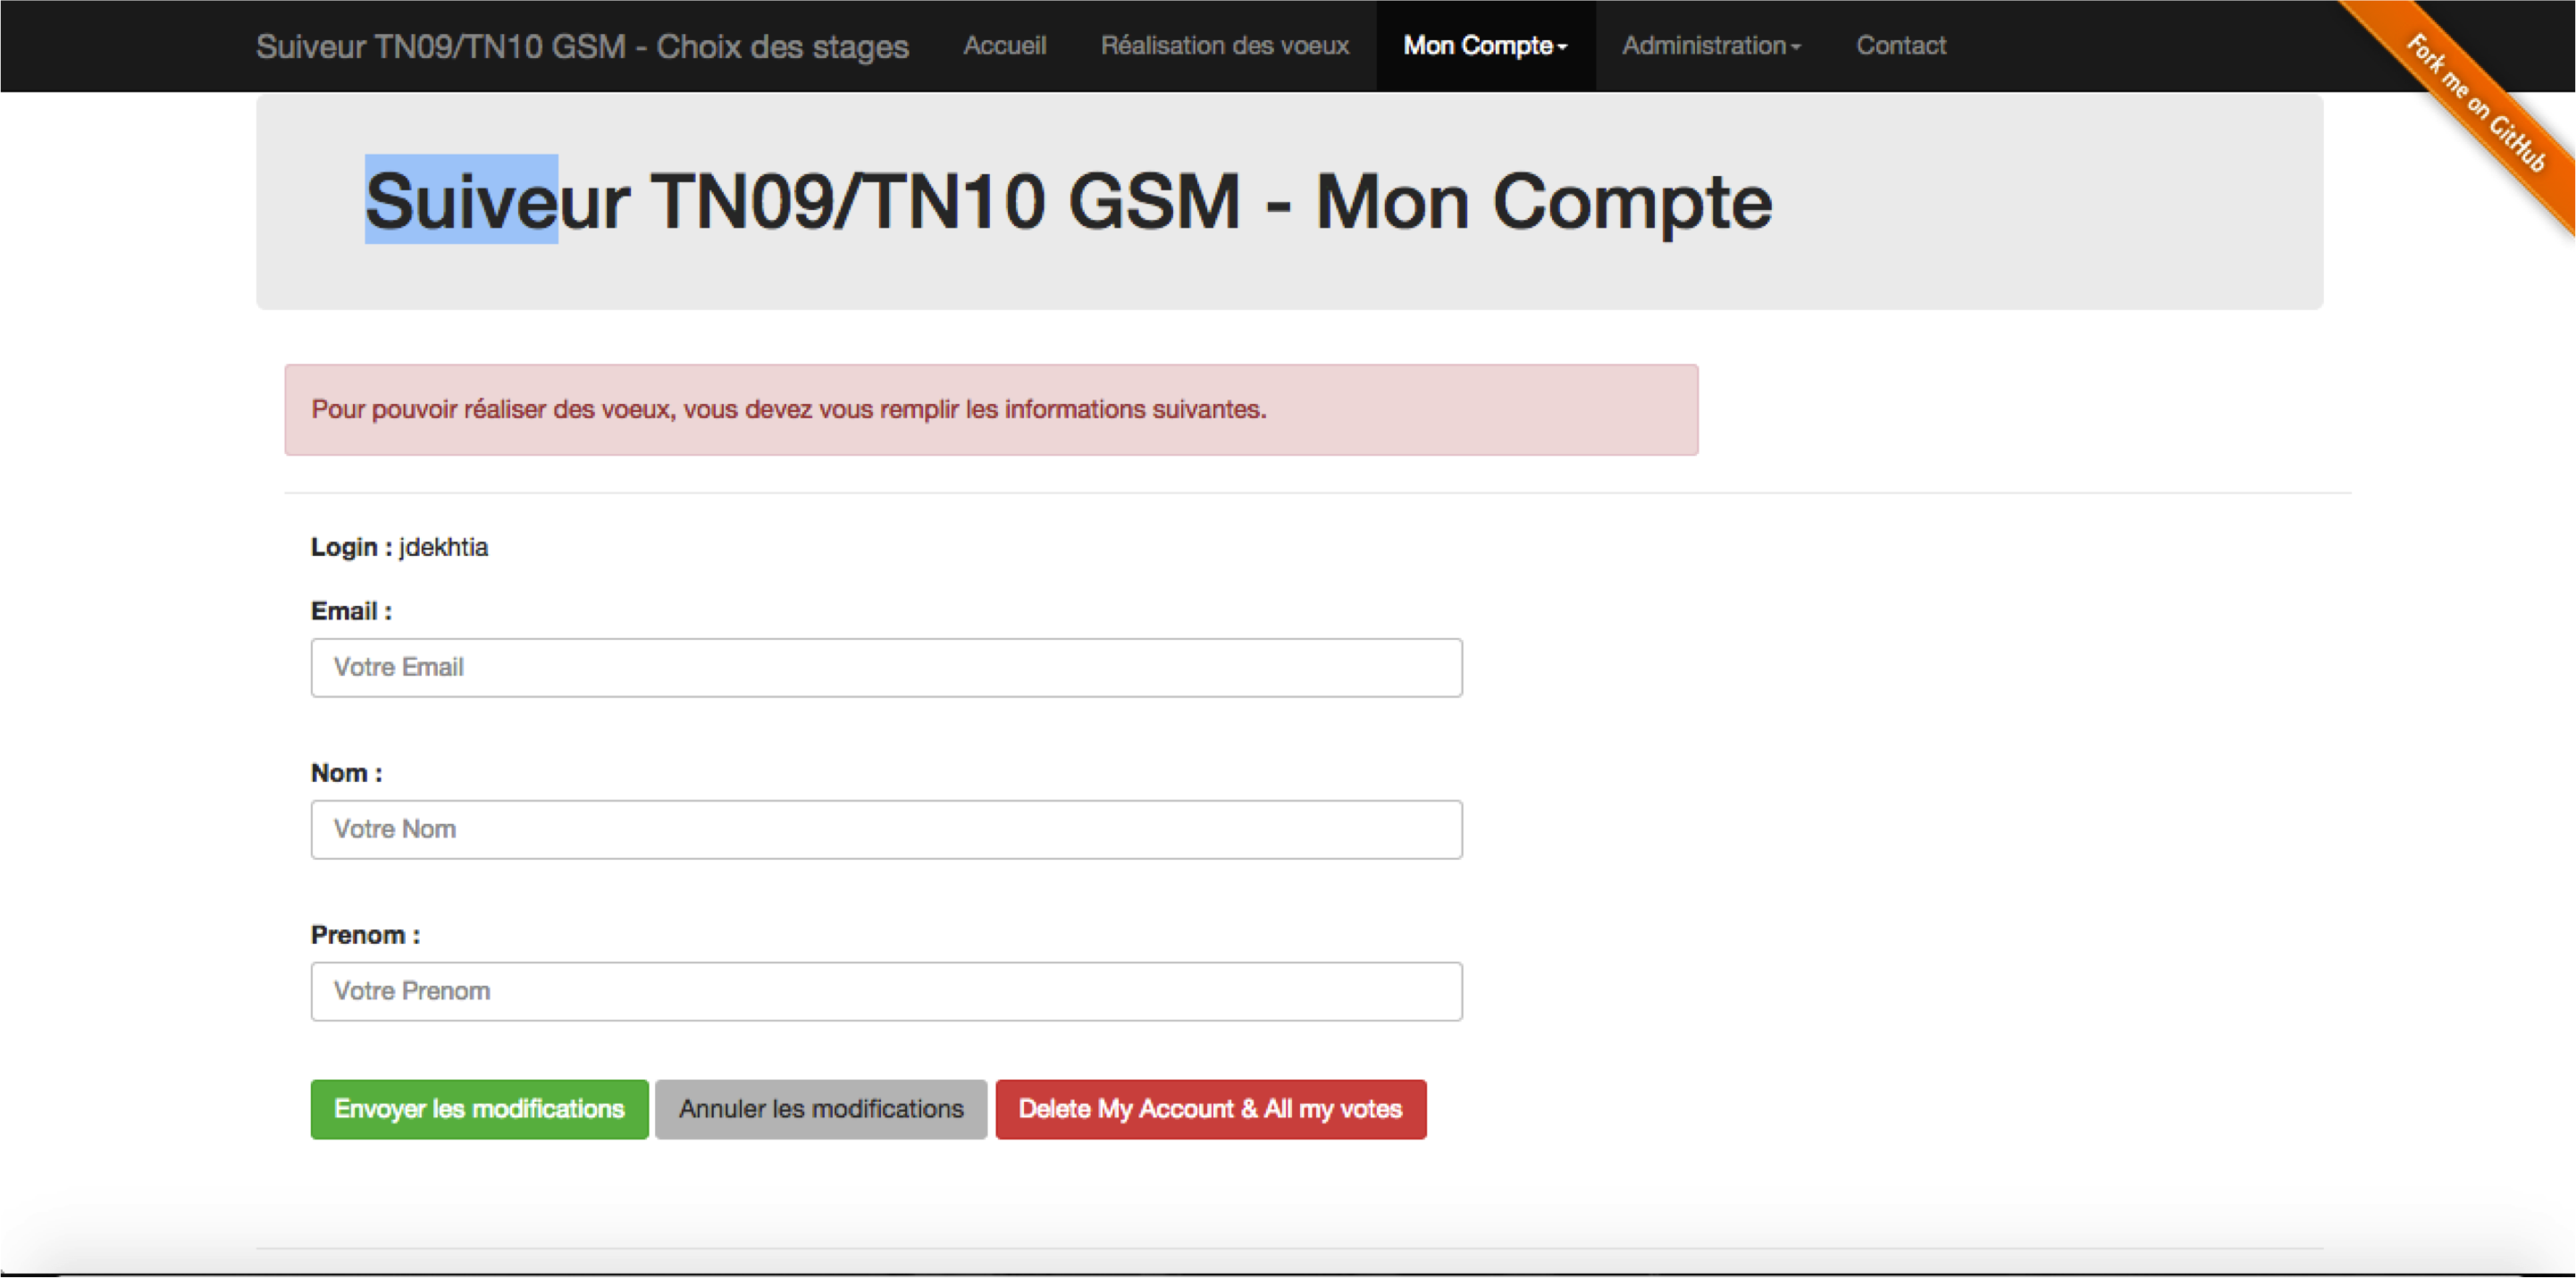
\includegraphics[scale=0.3]{Images/personal_infos.png}
		\caption{La page d'accueil - Renseignement des données personnelles}
	\end{center}
\end{figure}

Une fois les informations renseignées, et que vous avez cliqué sur "\textbf{envoyer les modifications}". La plateforme confirme la prise en compte des modifications.

\begin{figure}[H]
	\vspace{-3mm}
	\begin{center}
		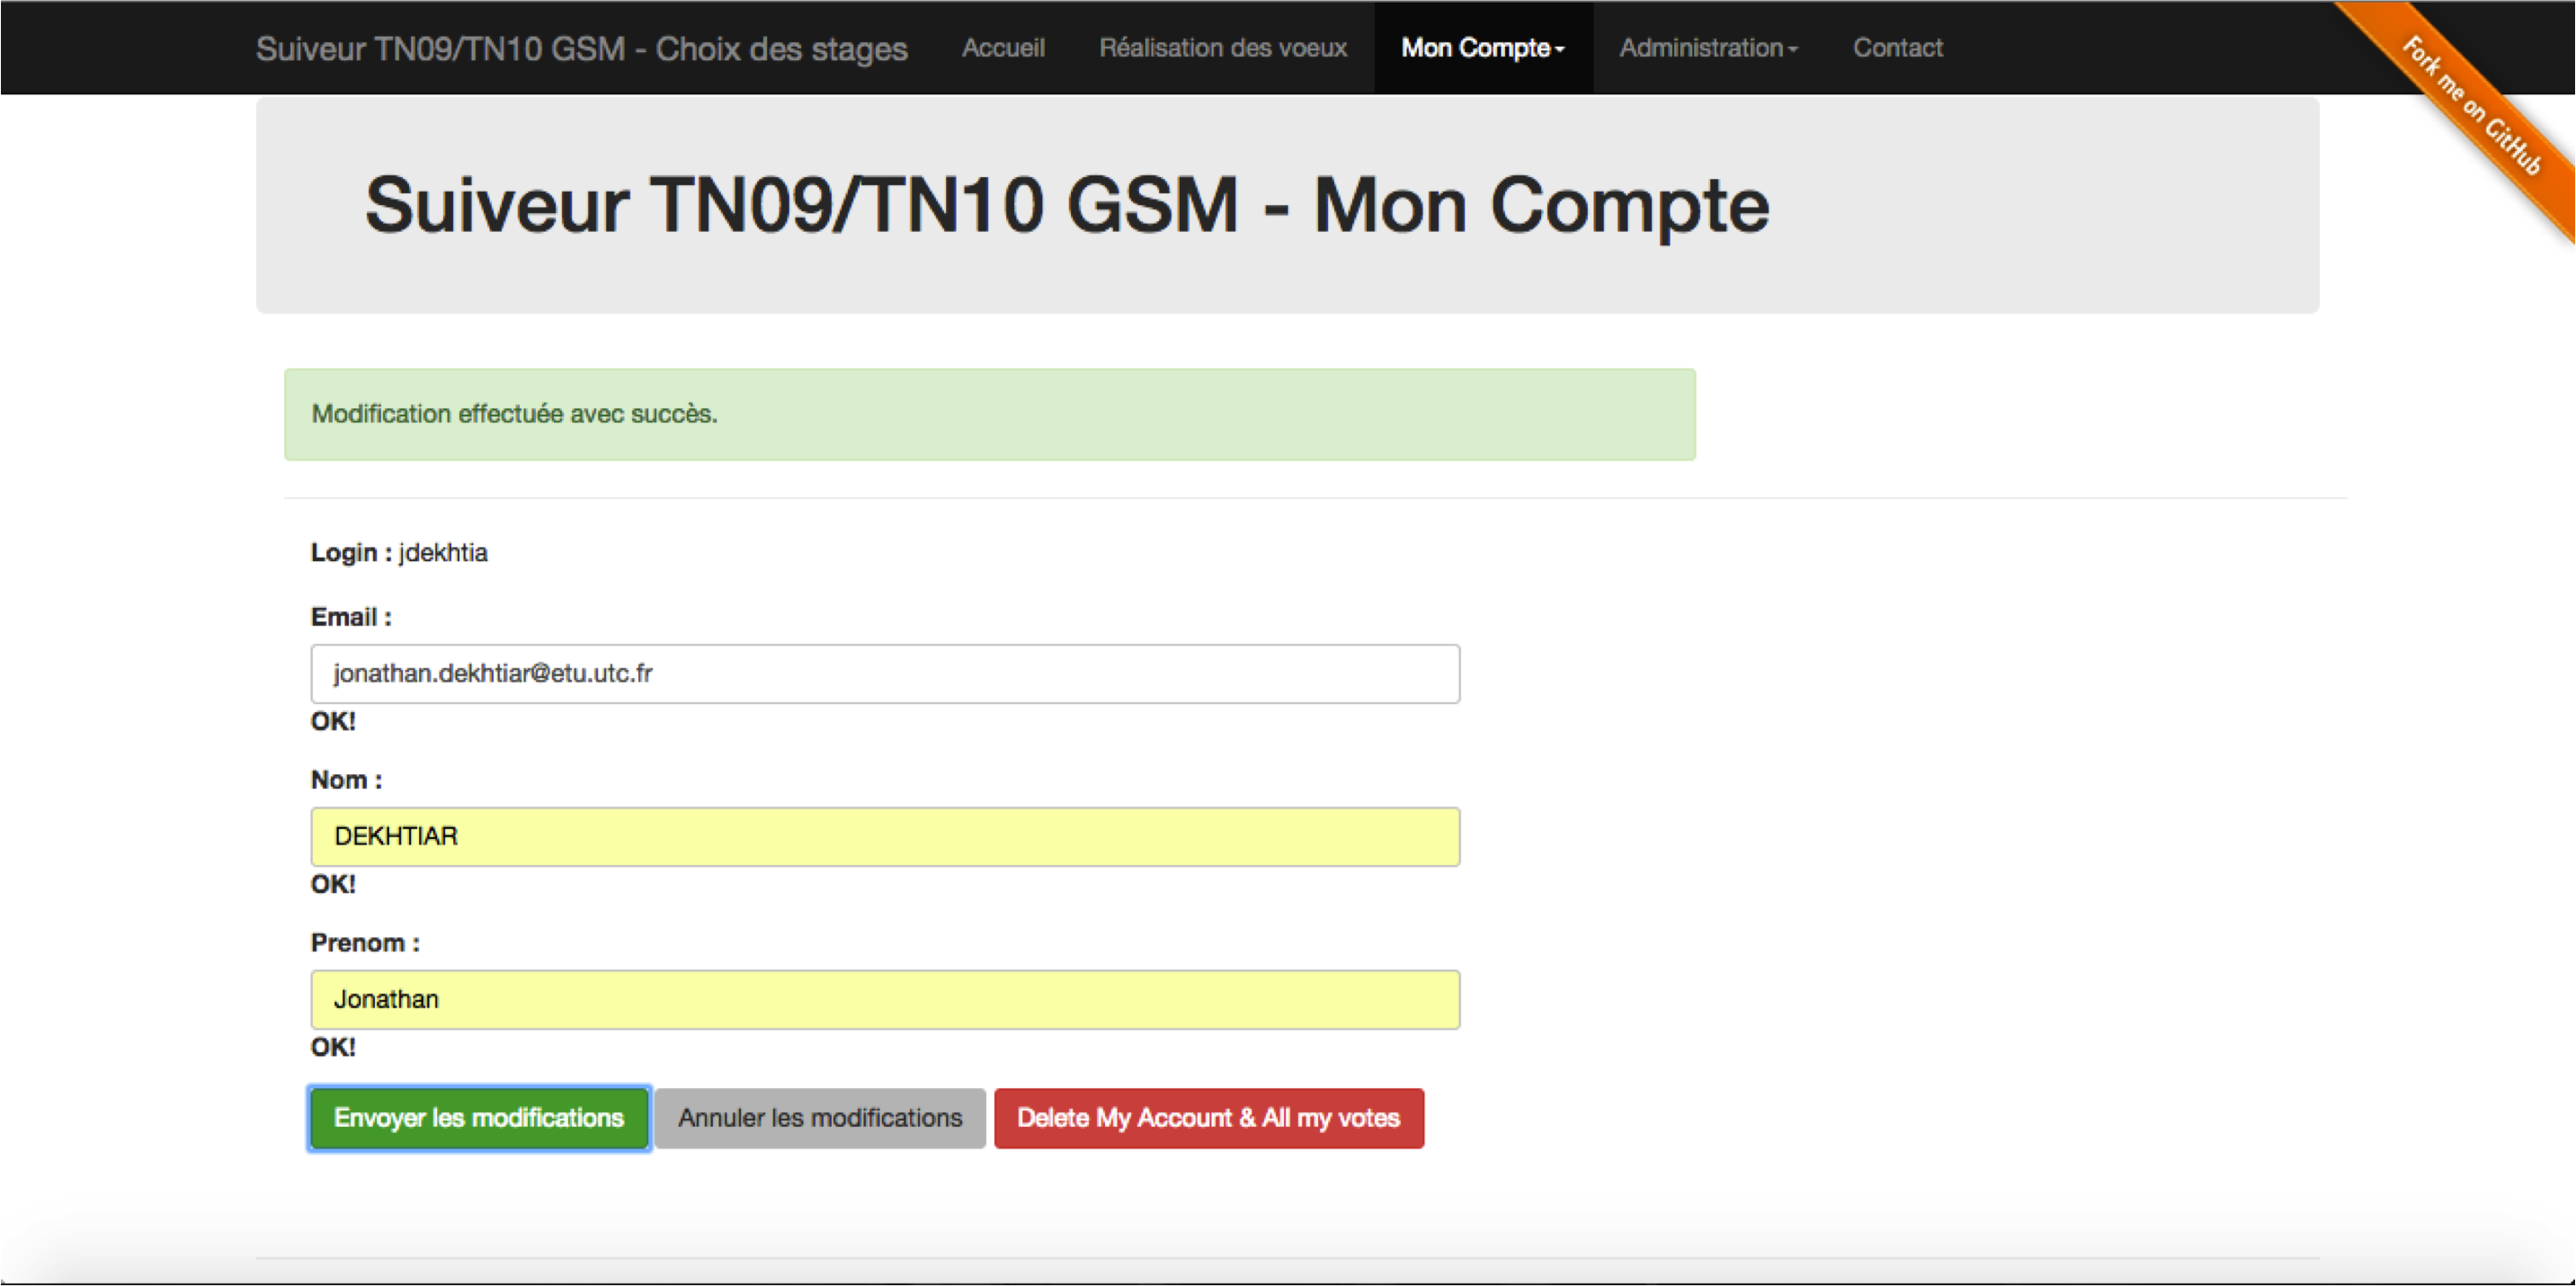
\includegraphics[scale=0.3]{Images/personal_infos_OK.png}
		\caption{La page d'accueil - Confirmation de prise en compte des renseignements}
	\end{center}
\end{figure}


Vous pouvez à tout moment remodifier ces informations ou supprimer votre compte en cliquant sur "\textbf{Mon Compte}" dans le menu, comme désigne la flèche rouge sur la capture d'écran suivante.\\

\textbf{Attention ! La suppression de votre compte supprimera également tous vos voeux et vos privilèges d'utilisateur.}\\

\begin{figure}[H]
	\vspace{-3mm}
	\begin{center}
		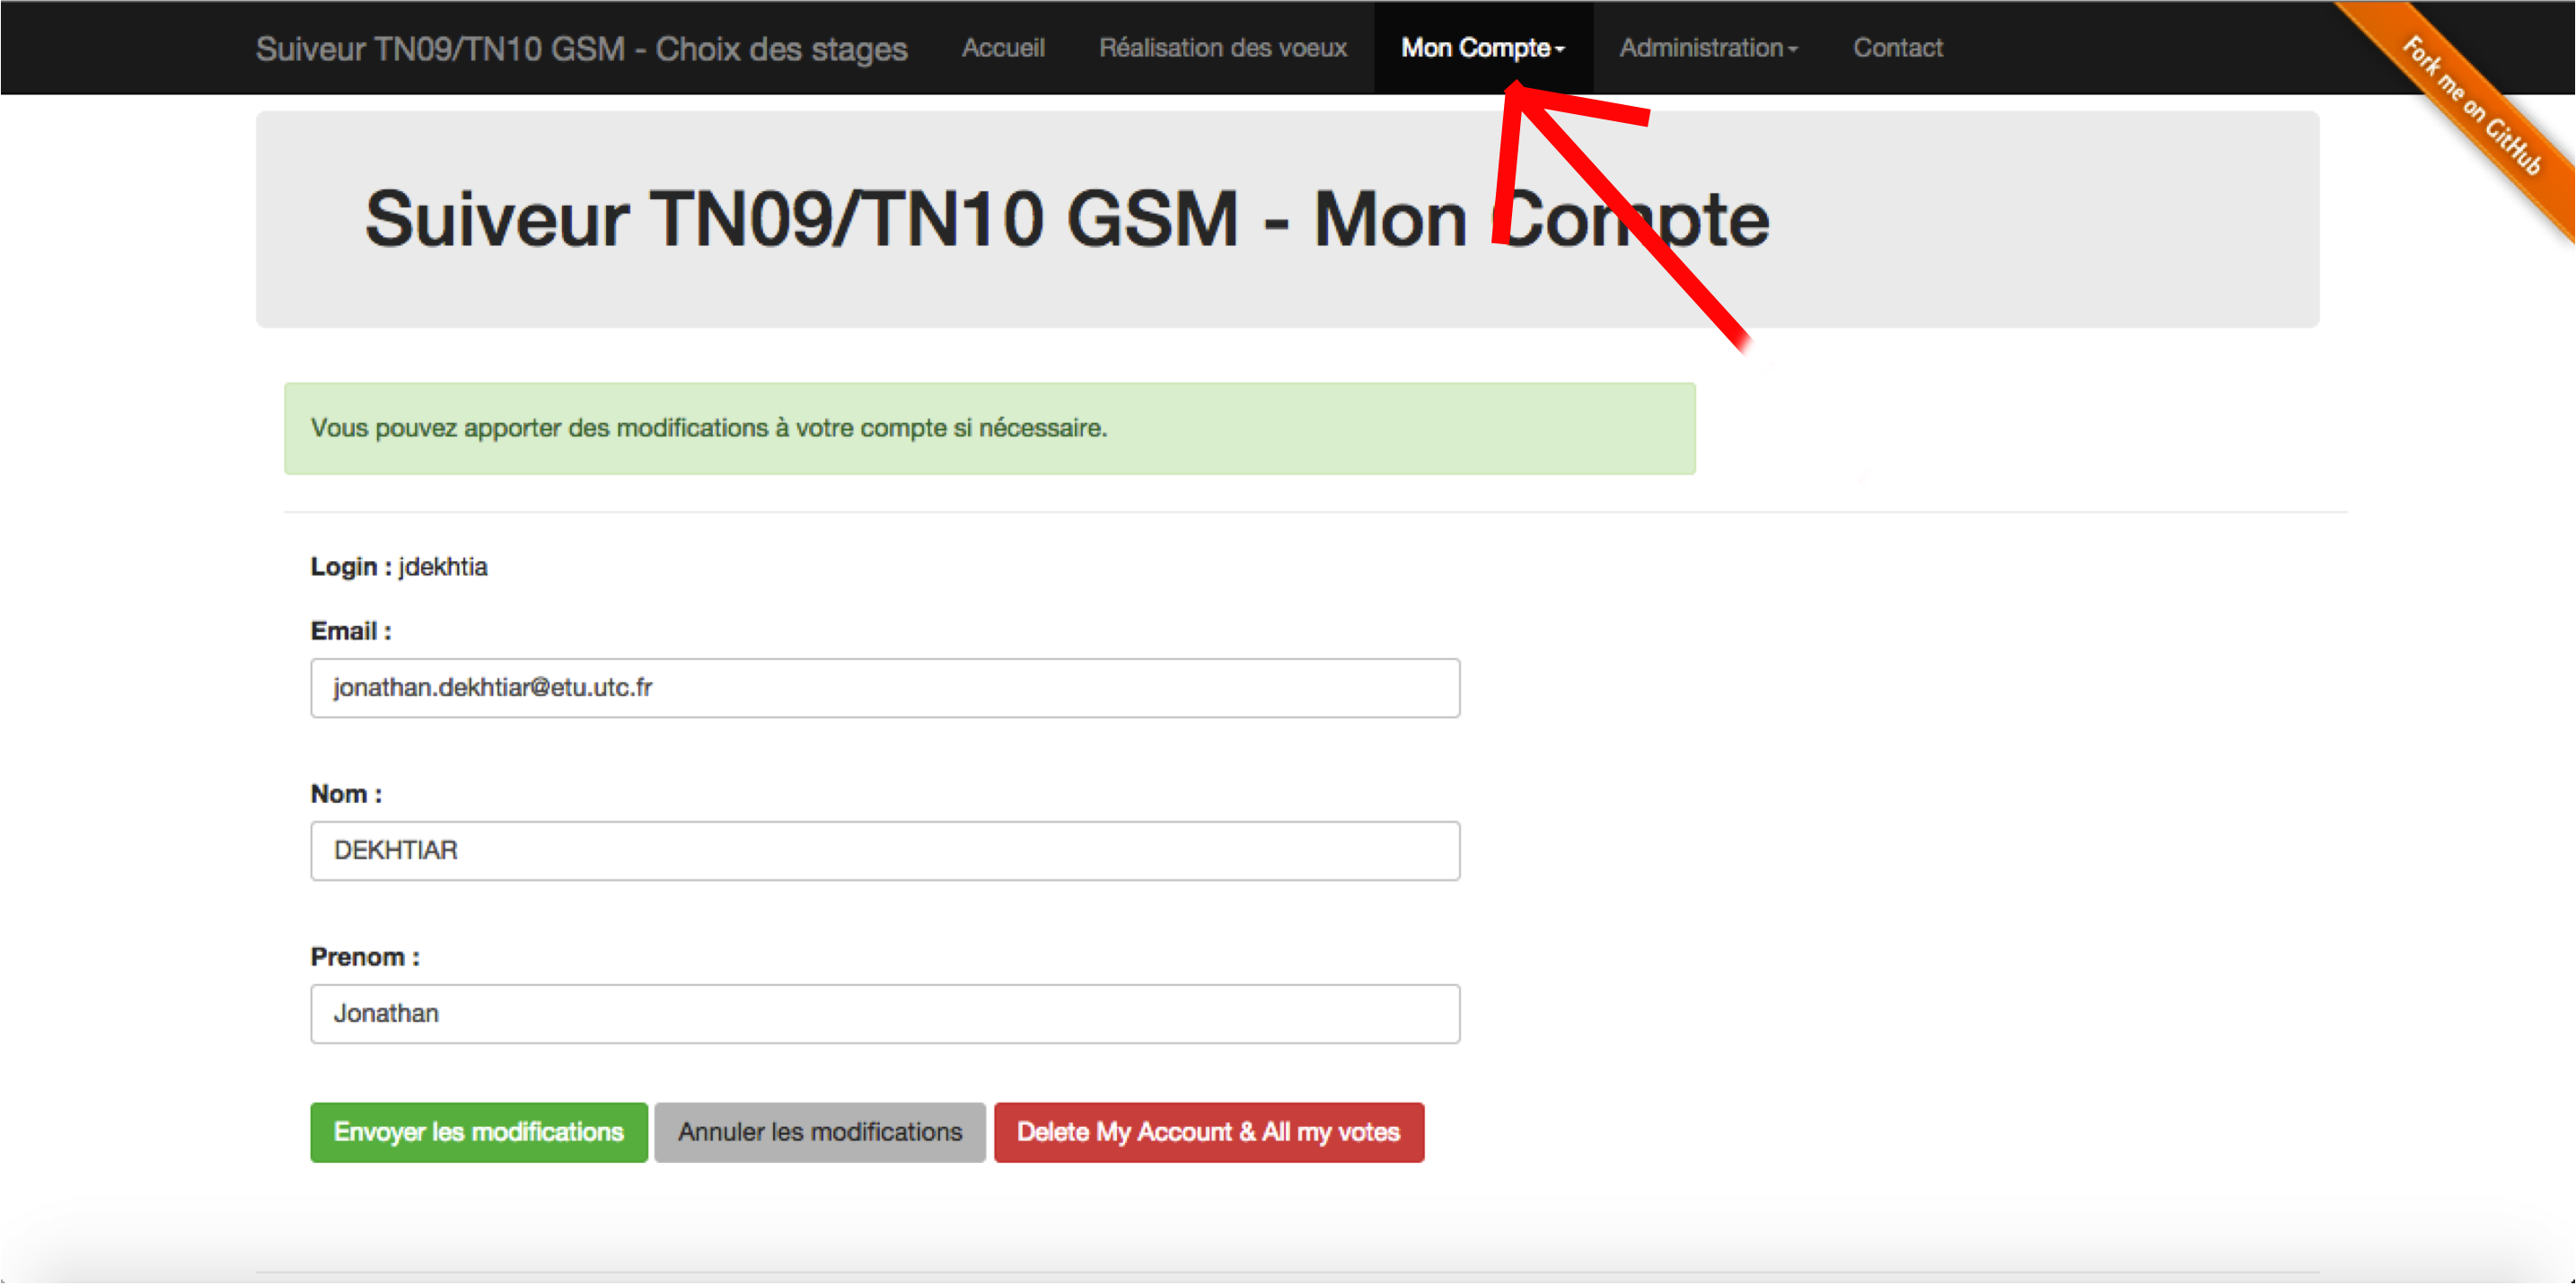
\includegraphics[scale=0.3]{Images/personal_infos_modif.png}
		\caption{Modification de son compte personnel}
	\end{center}
	\vspace{-1.5cm}
\end{figure}

\clearpage


\subsection{Réalisation des voeux}

En cliquant sur l'onglet "\textbf{Réalisation des voeux}", on accède au panneau de vote.\\

On y retrouve les informations clés suivantes :\\
\begin{itemize}
	\item Numéro du Stage
	
	\item Type de Stage
	
	\item Ville
	
	\item Titre du Stage
	
	\item Nom de l'entreprise
	
	\item Un lien vers la description complète du stage
	
	\item Le \textbf{widget} de notation\\
	
\end{itemize}

\begin{figure}[H]
	\vspace{-3mm}
	\begin{center}
		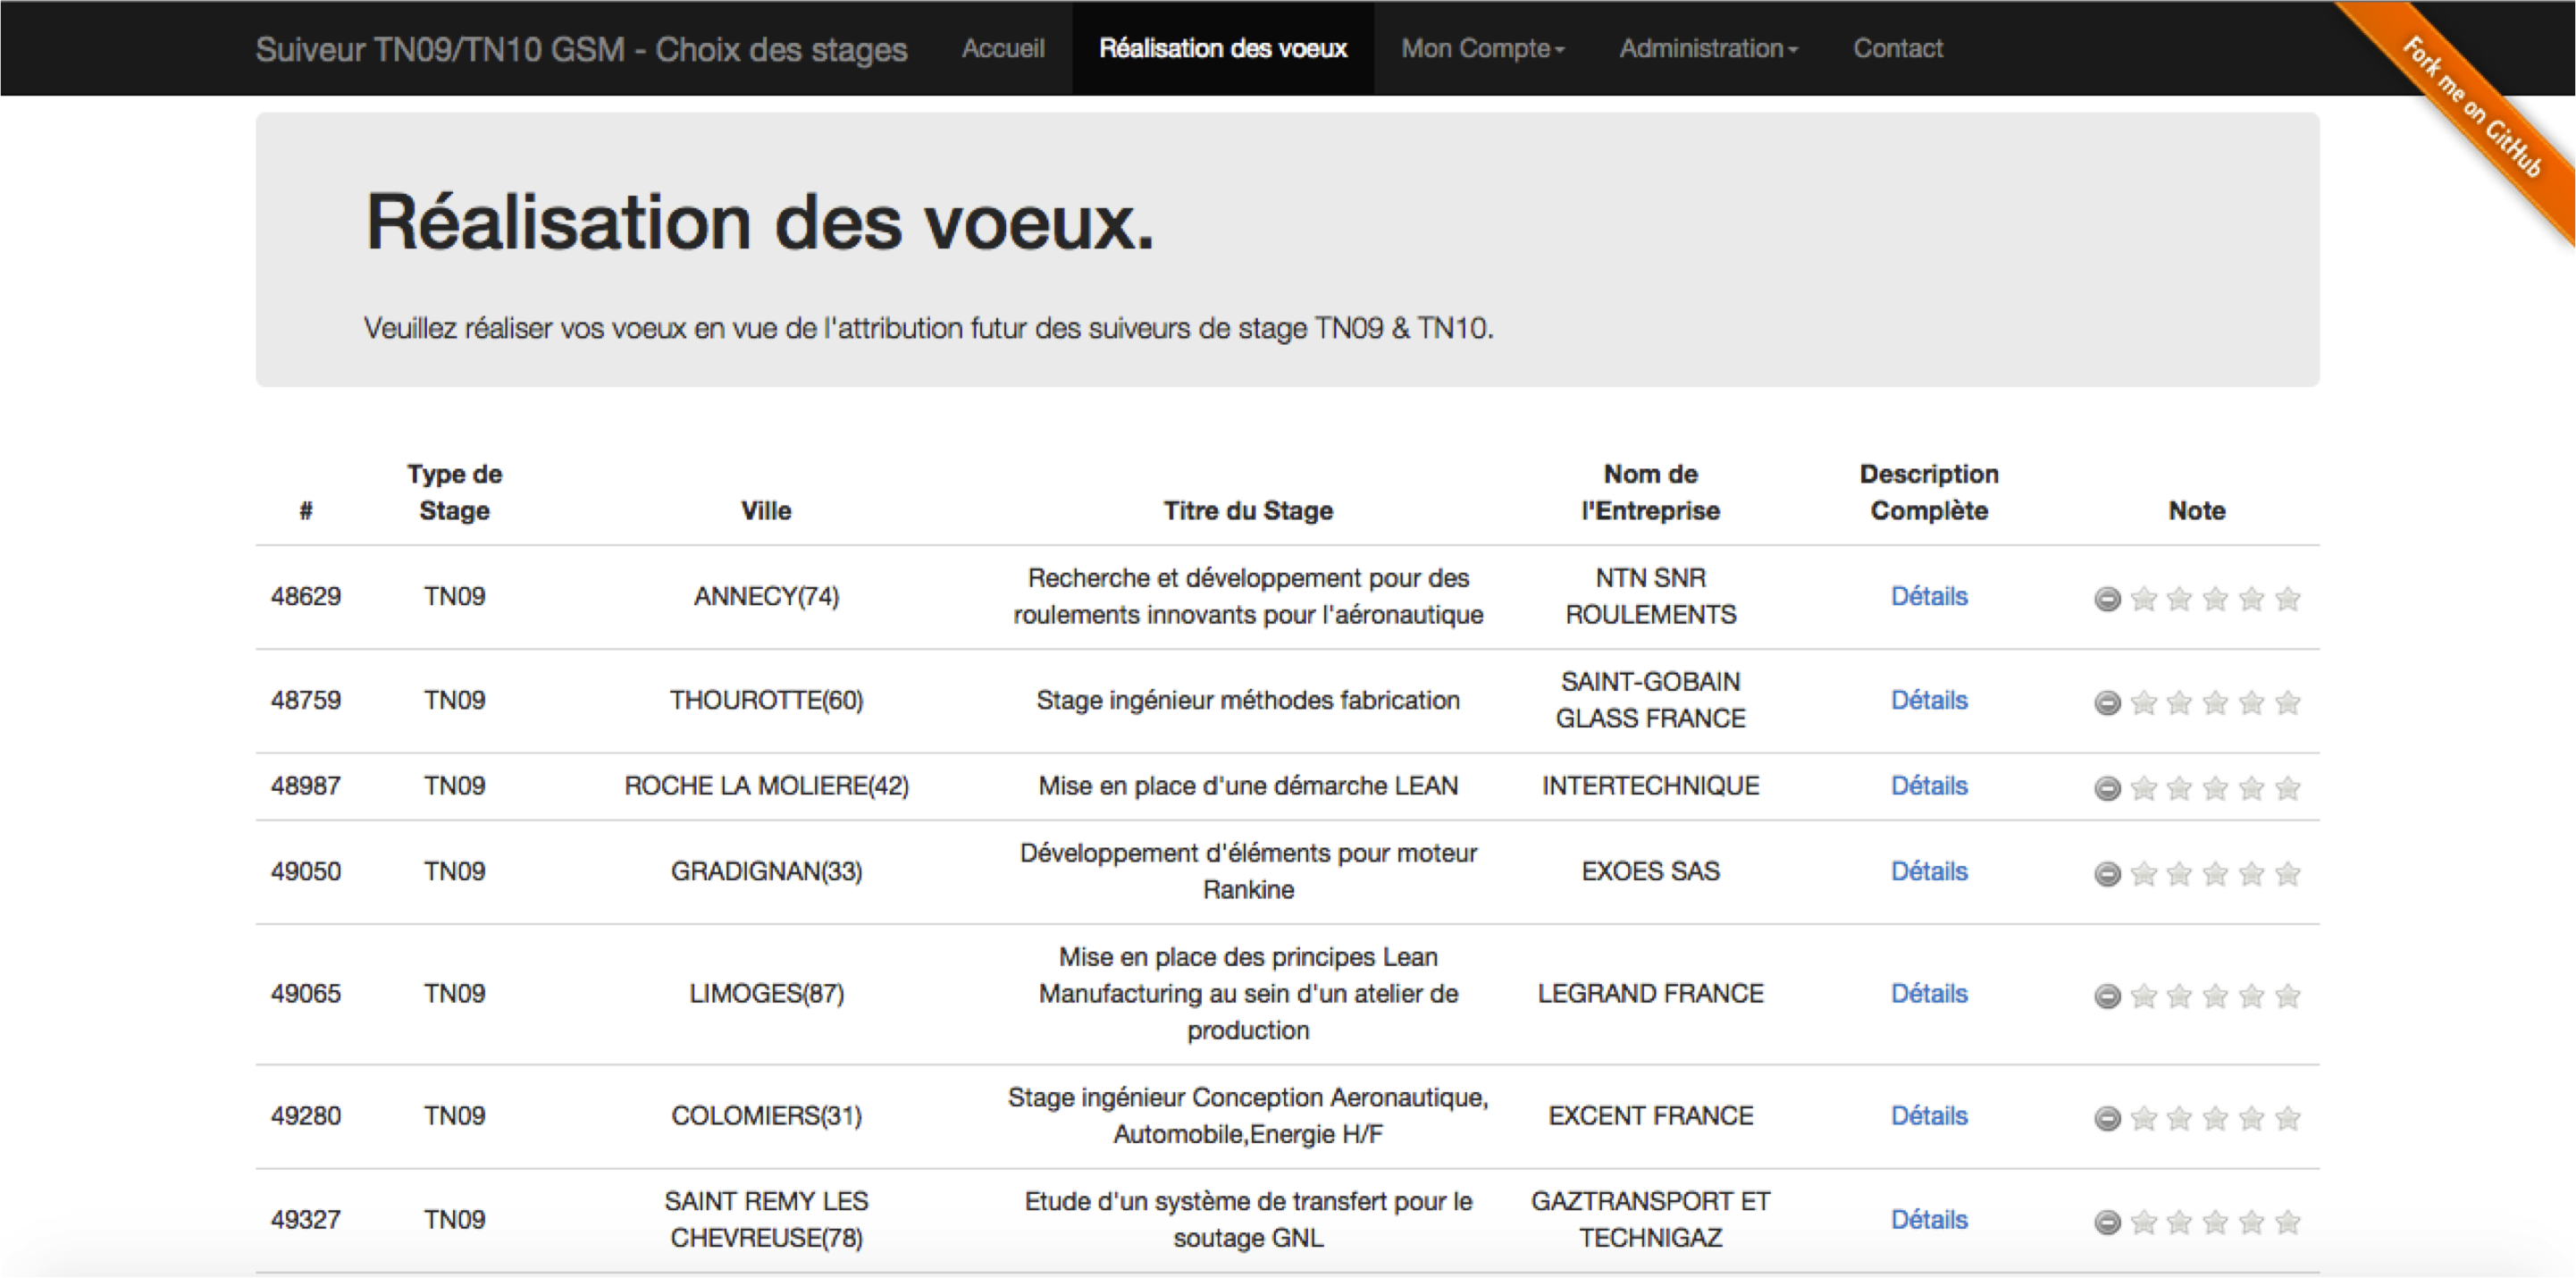
\includegraphics[scale=0.31]{Images/vote_1.png}
		\caption{La page des votes}
	\end{center}
\end{figure}



\subsubsection{Le Widget de Vote}

Le widget de vote fonctionne de la manière suivante :\\

\begin{itemize}
	\item On clique sur le nombre d'étoiles que l'on veut attribuer.
	
	\item Pour modifier, il suffit de cliquer sur le nouveau nombre d'étoiles que l'on veut attribuer.
	
	\item 5 étoiles représentes la note maximale, 1 étoile la note minimale, 0 étoile signifie que vous n'en voulez pas.
	
	\item Pour supprimer un vote et retourner à 0 étoile, il faut cliquer sur le panneau \textbf{sens interdit}.
	
	\item Les votes sont automatiquement enregistrés, inutile de chercher comment sauvegarder.
\end{itemize}


\subsubsection{Rafraichissement de la page des votes}

Lors du rafraichissement de la page, si des voeux ont été réalisés, alors ces stages apparaissent en premier et classés par note attribuée en ordre décroissant (les notes les plus élevée en première).\\
Les autres stages restent classés par \textbf{numéro de stage}.\\

\begin{figure}[H]
	\vspace{-3mm}
	\begin{center}
		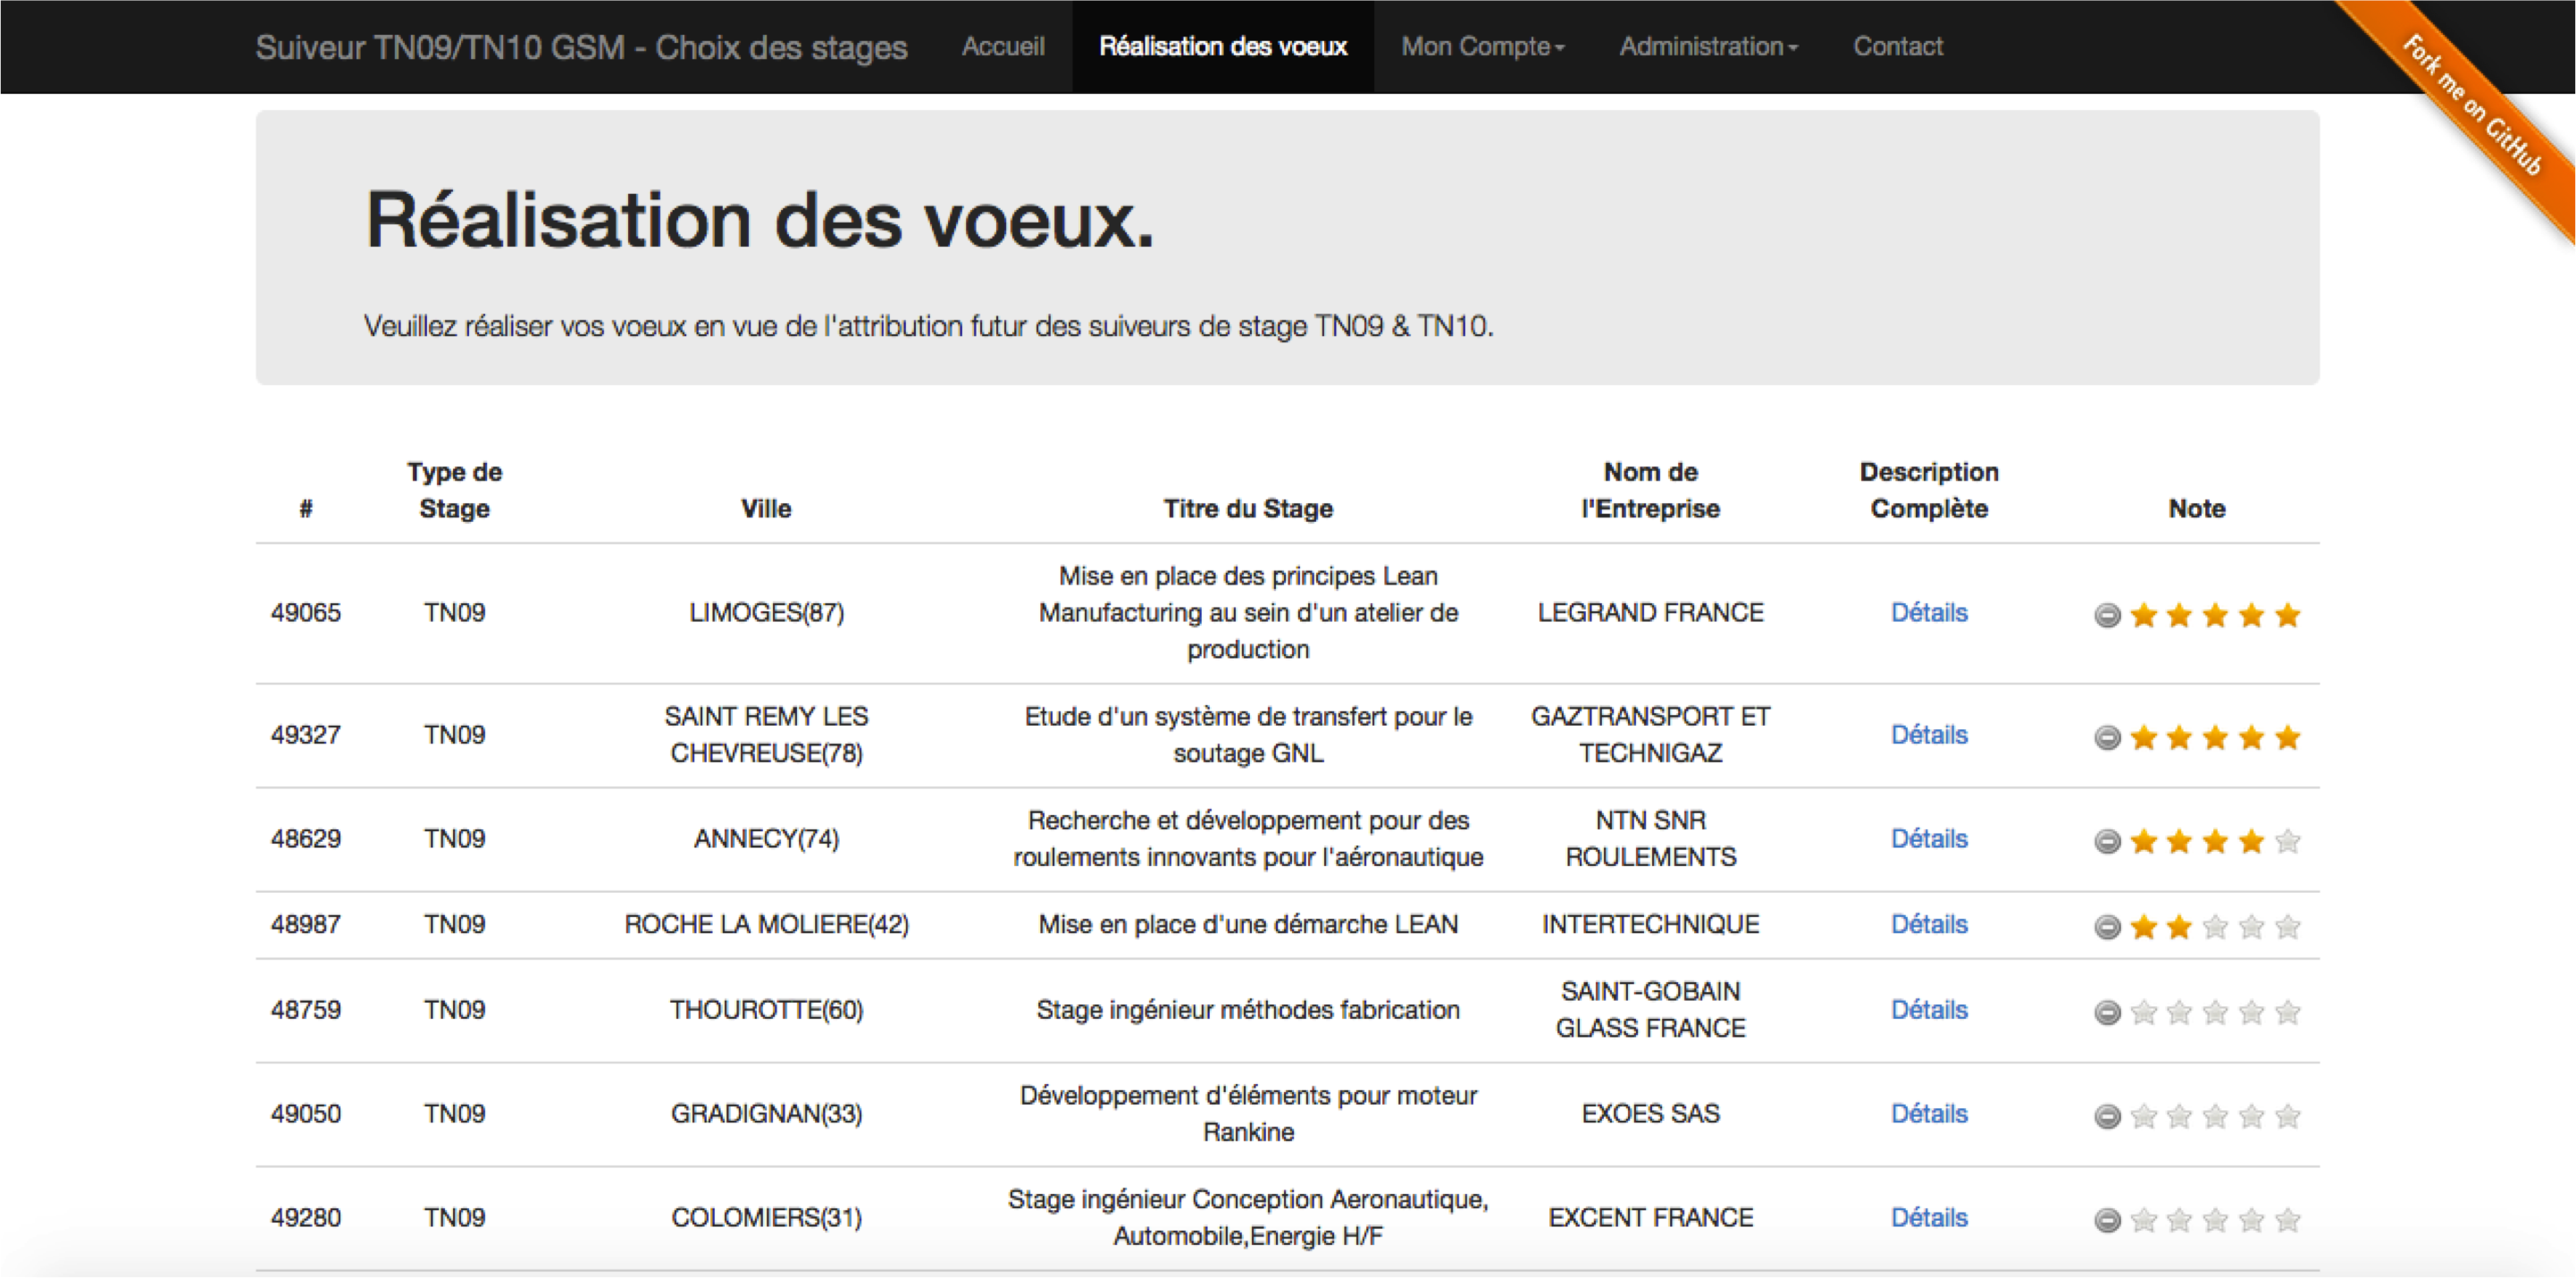
\includegraphics[scale=0.3]{Images/vote_2.png}
		\caption{La page des votes - Votes déjà effectués}
	\end{center}
\end{figure}

\subsubsection{L'onglet "Détails"}

Si l'on clique sur le lien "\textbf{Détails}", une fenêtre est chargé en \textbf{AJAX} et affiche la totalité des informations concernant le stage.\\
L'avantage de l'utilisation de l'AJAX est qu'aucune nouvelle page est chargé, la plateforme doit rester le plus \textbf{fluide et dynamique} possible.\\

\begin{figure}[H]
	\vspace{-3mm}
	\begin{center}
		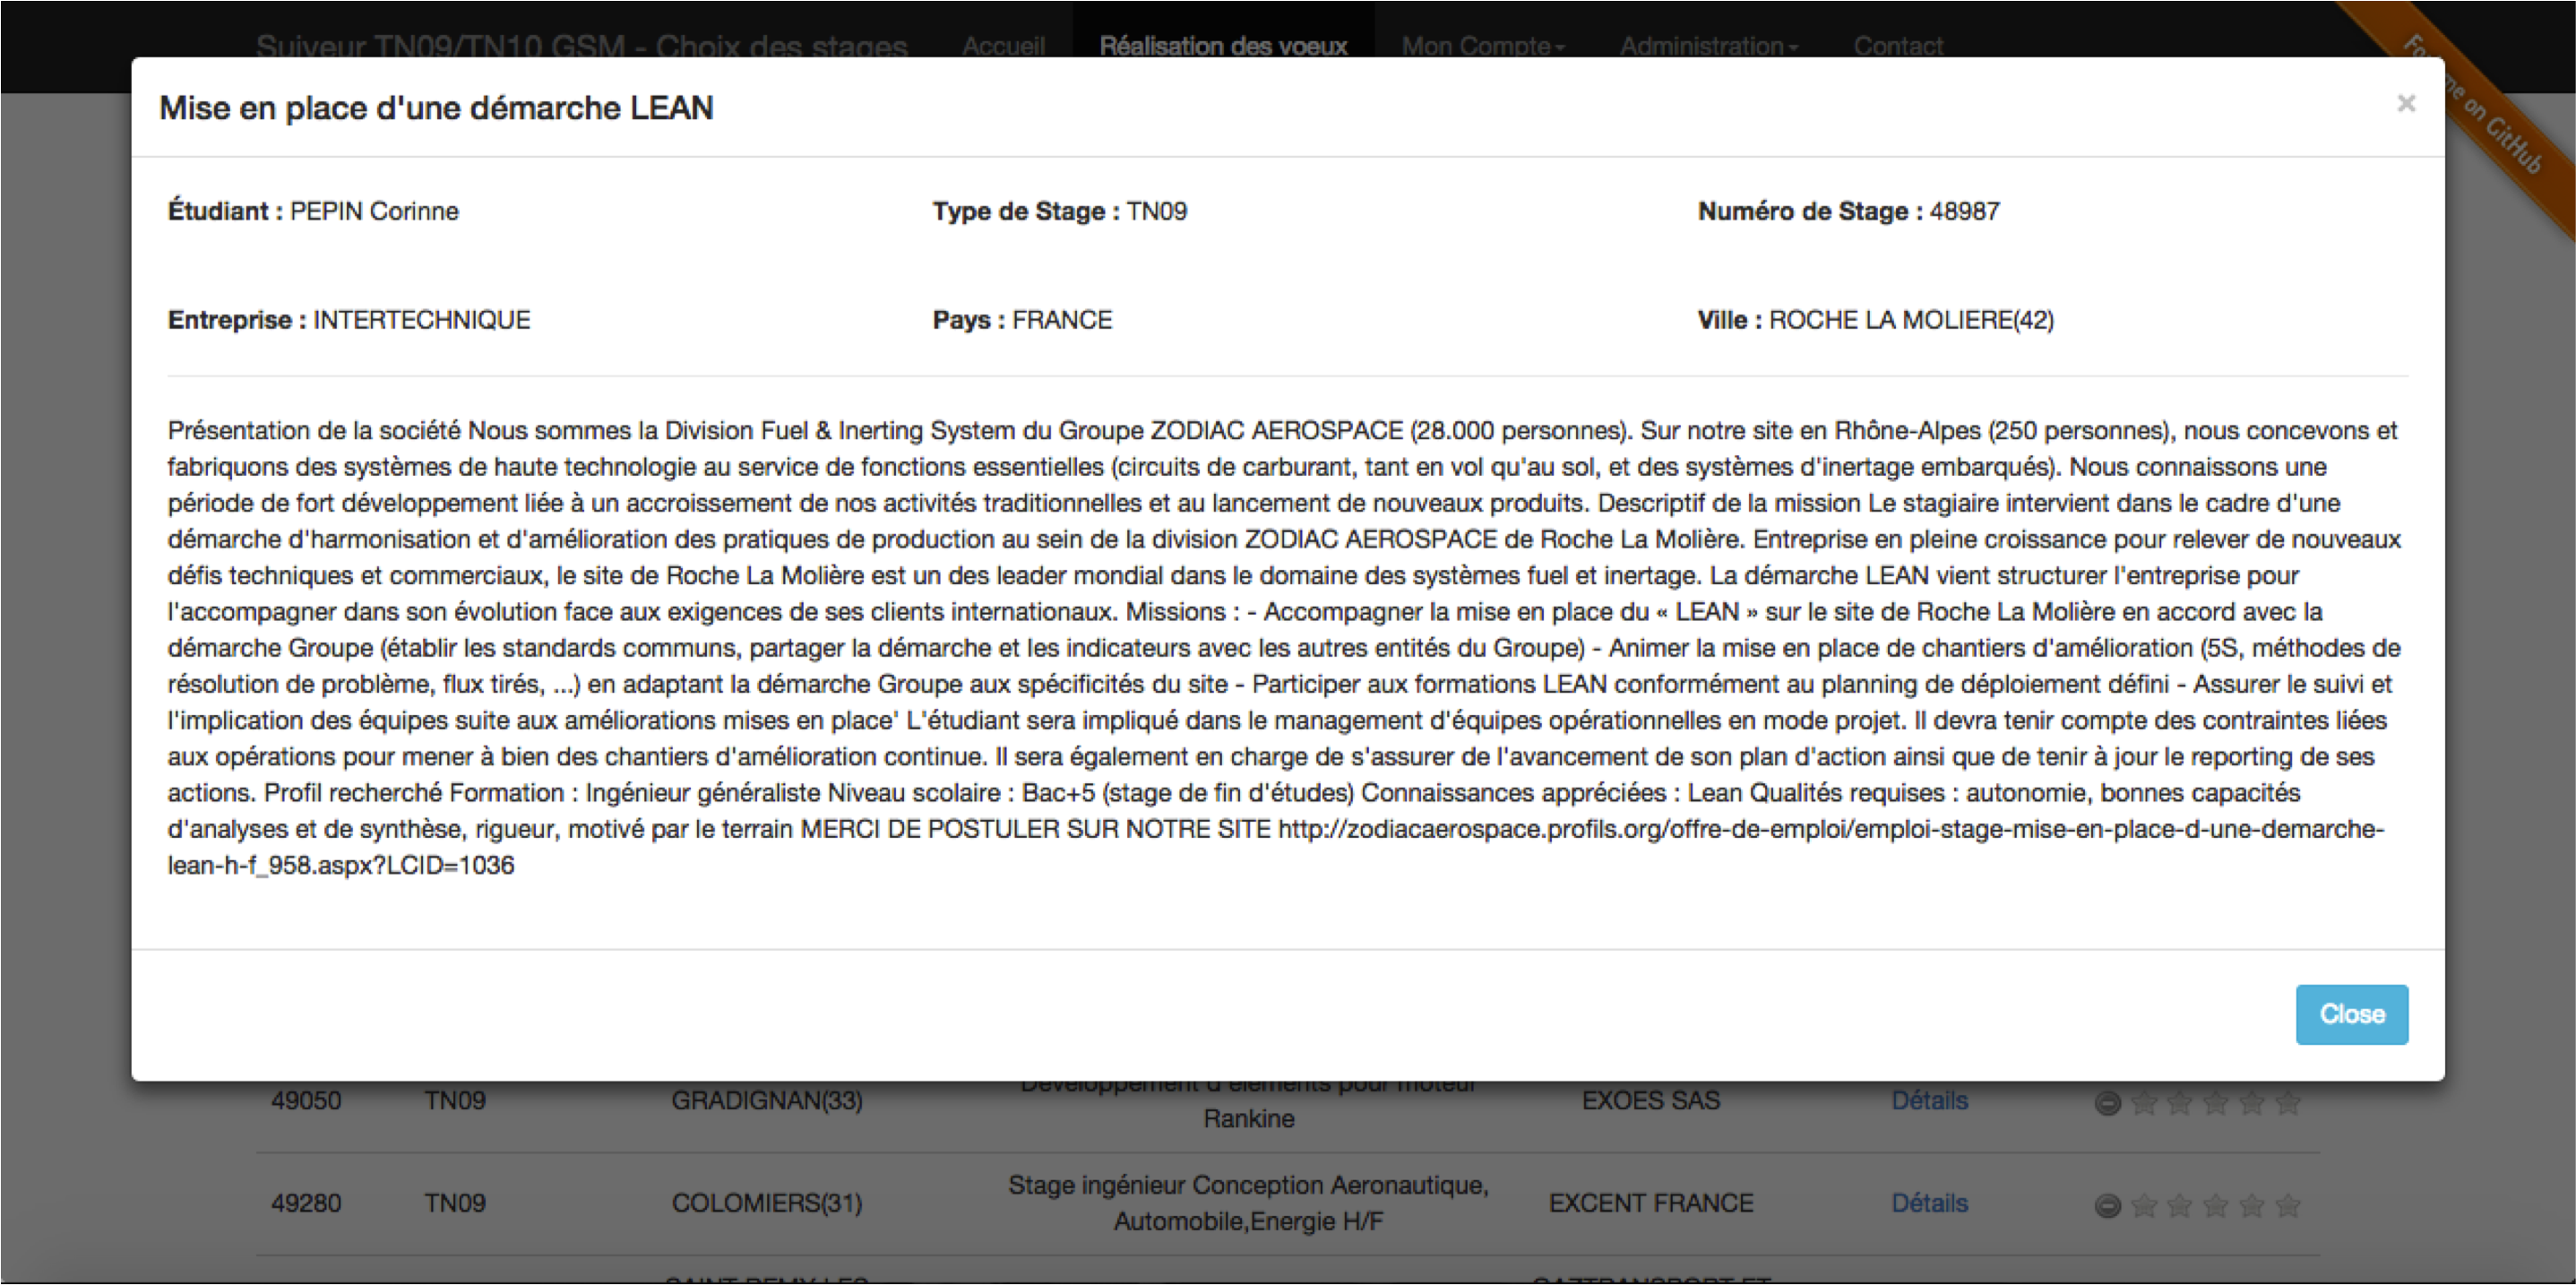
\includegraphics[scale=0.3]{Images/vote_detail.png}
		\caption{La page des votes - Votes déjà effectués}
	\end{center}
	\vspace{-2cm}
\end{figure}

\clearpage

\subsection{Le formulaire de Contact}

Le formulaire de contact permet à tout utilisateur de contacter les administrateurs et les assistants afin de leur relater un problème.\\

Tous reçoivent le message, ce qui permet de ne pas avoir à changer le nom manuellement de celui en charge de recevoir les emails, cela permet de palier aux différents congés, maladies, déplacements, indisponibilités.\\

\begin{figure}[H]
	\vspace{-3mm}
	\begin{center}
		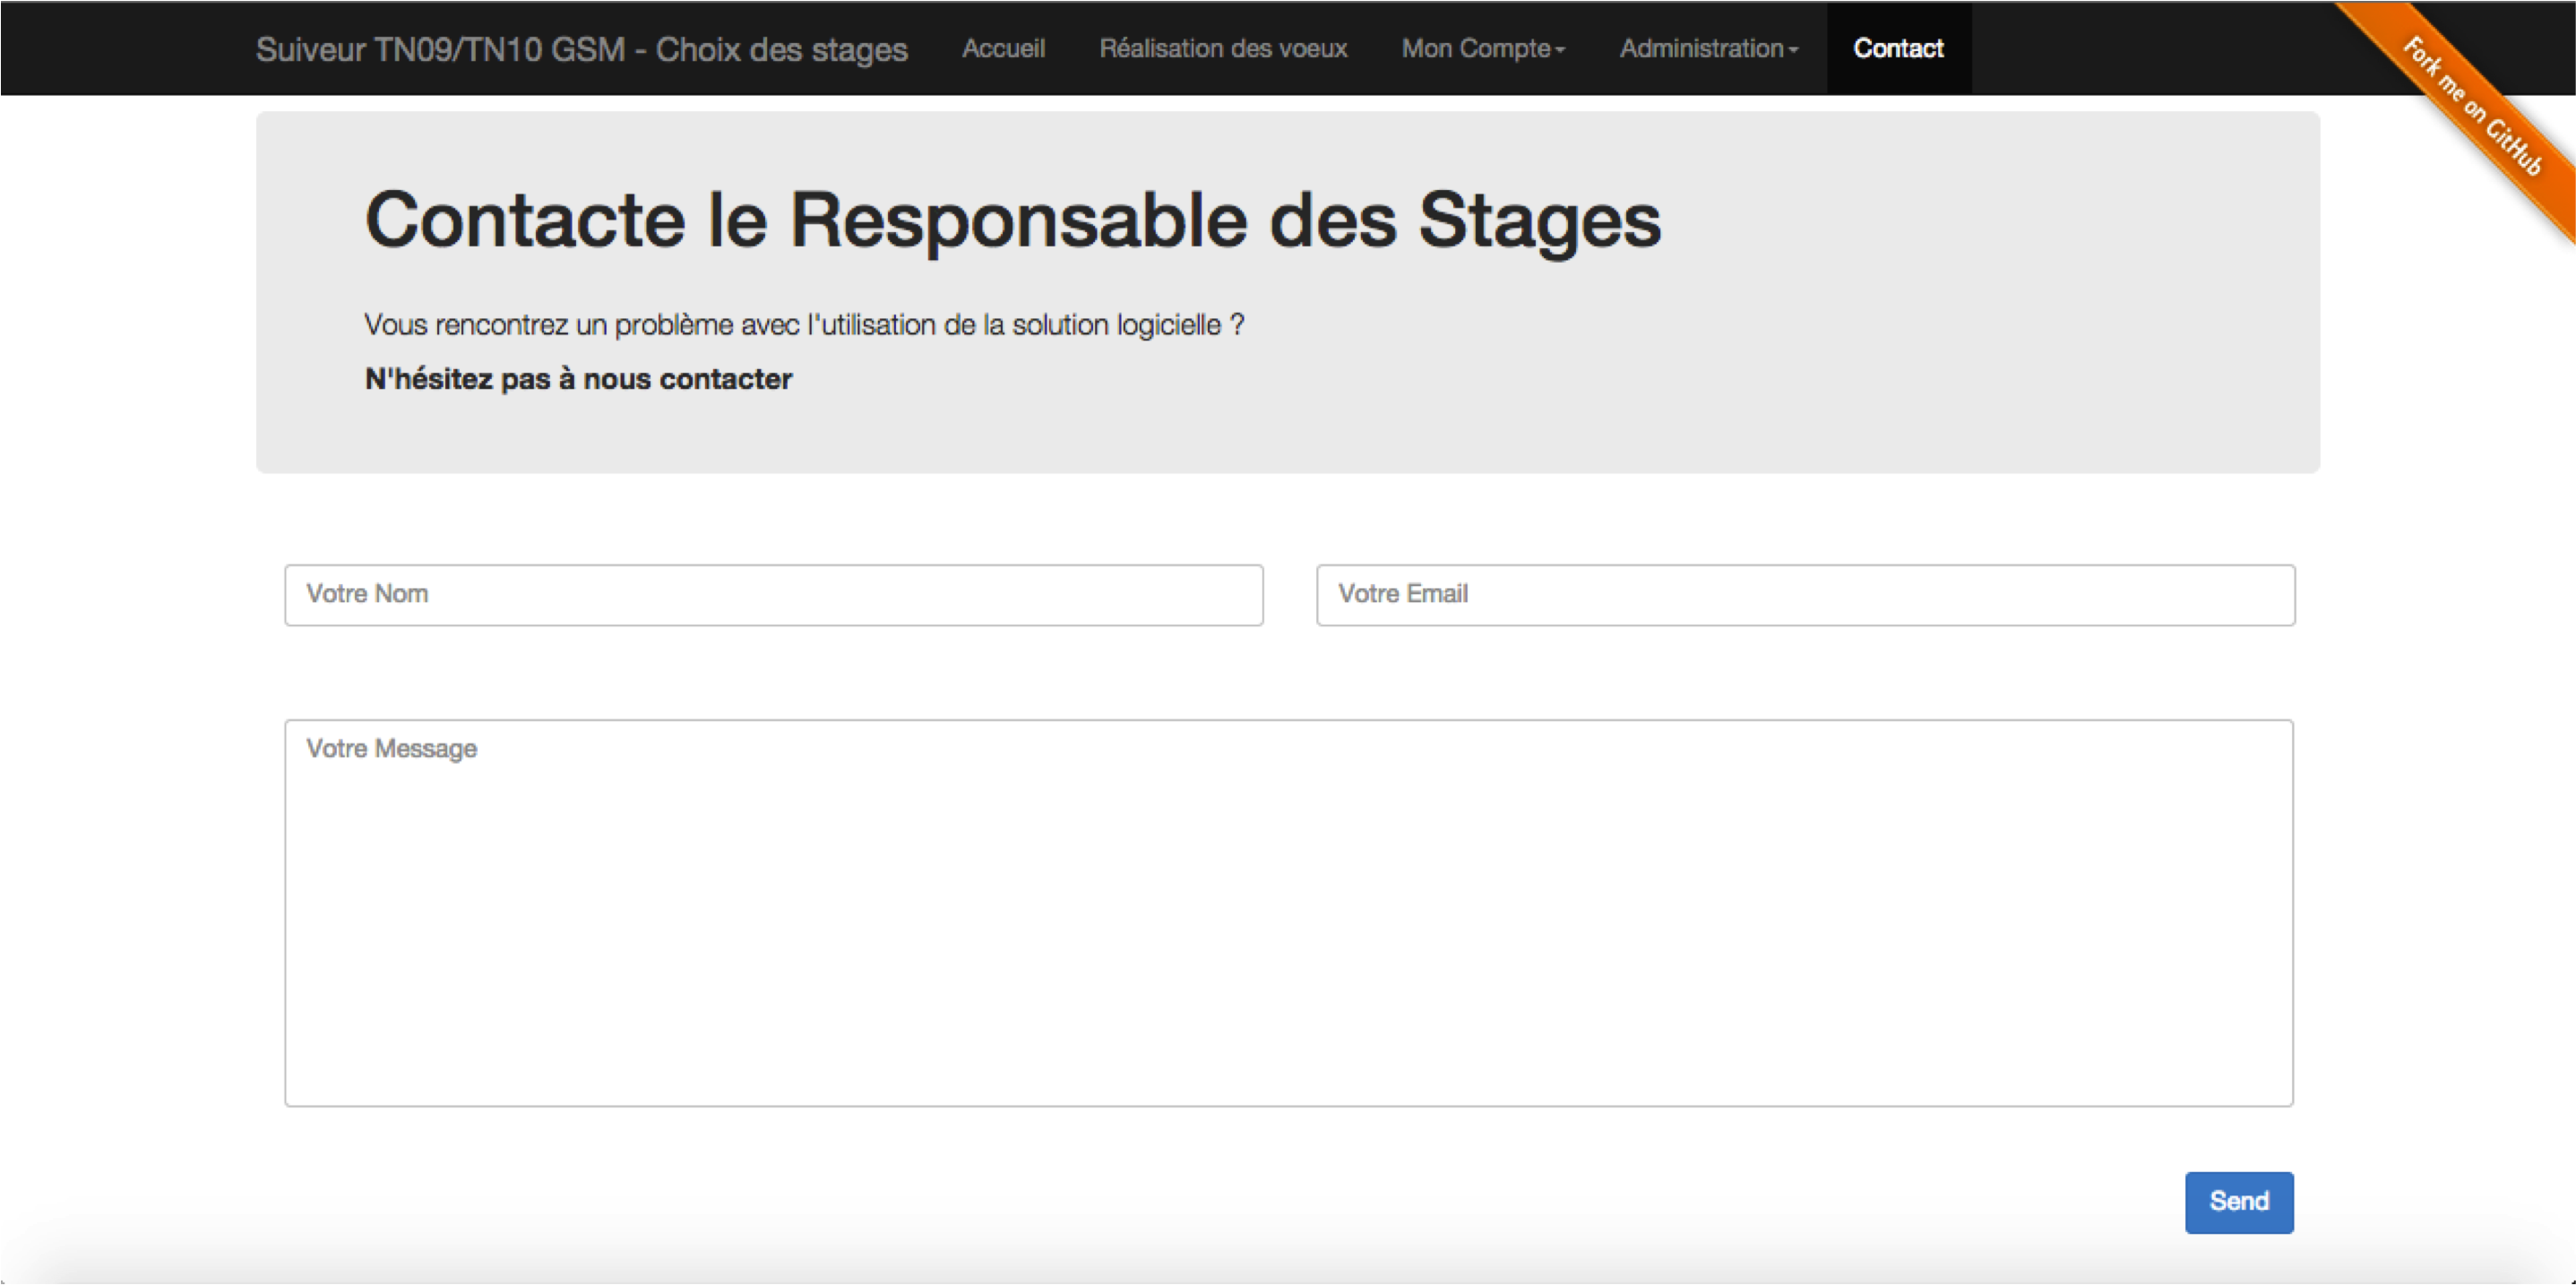
\includegraphics[scale=0.3]{Images/contact.png}
		\caption{La page des votes - Votes déjà effectués}
	\end{center}
\end{figure}

\clearpage

%------------------------------------------------------------------------------

\section{Utilisation de la plateforme - Point de vue Administrateur}

\subsection{Les différents droits d'accès}

Évidement, tout le monde ne peut accéder à la partie d'administration.\\

Plusieurs droits d'accès ont été établis : \\

\begin{itemize}
	\item \textbf{Utilisateur :} Droit par défaut. Il peut modifier son compte, n'a pas accès à toute la partie d'administration.\\
	
	\item  \textbf{Assistant :} En plus des droits de l'utilisateur classique, possibilité de tout effectuer en administration sauf le management des droits d'accès.\\
	
	\item \textbf{Administrateur :} Ce dernier a tous les droits, seul droit d'accès permettant de modifier les droits d'accès.\\
	
	
\end{itemize}

Chacun des droits peut être donné à plusieurs personnes. (\textit{Exemple :} il peut y avoir deux administrateurs).\\

\textbf{Remarque : }Tous les administrateurs et les assistants reçoivent les emails envoyé depuis le formulaire de contact.\\

\begin{figure}[H]
	\vspace{-3mm}
	\begin{center}
		
\includegraphics[scale=0.47]{Images/admin_menu.png}
		\caption{Menu d'administration}
	\end{center}
\end{figure}


\begin{figure}[H]
	\vspace{-3mm}
	\begin{center}
		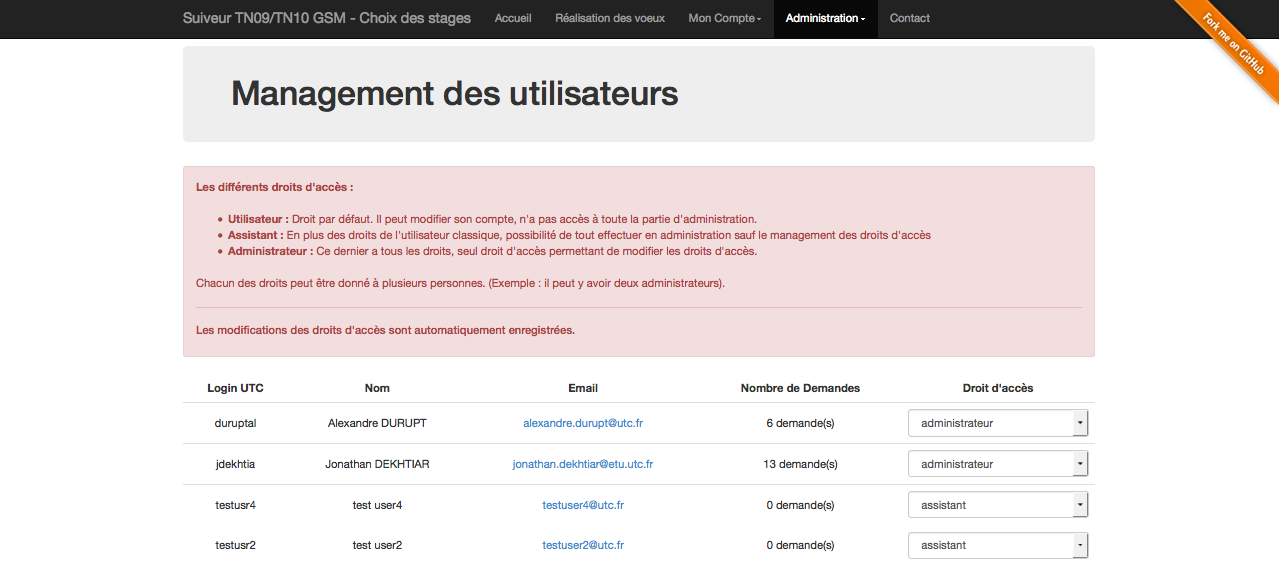
\includegraphics[scale=0.33]{Images/rights_management.png}
		\caption{Panneau de gestion des droits d'utilisateur.}
		\vspace{-2cm}
	\end{center}
\end{figure}

\clearpage

Pareillement les droits d'accès sont automatiquement sauvegardés lors du changement des droits. On peut également voir sur ce panneau, le nombre de vote par personne.\\

Il est à noter que seul les administrateurs peuvent changer les droits d'accès à la plateforme. Il est strictement impossible de changer son propre droit d'accès à la plateforme, même si on est administrateur. Ceci pour éviter de supprimer tous les administrateurs de la plateforme.\\
Cependant un administrateur peut modifier les droits de tous les autres administrateurs. Ce qui \textit{"passer le flambeau"} entre administrateur.

\subsection{Import des stages dans le système}

\begin{figure}[H]
	\vspace{-3mm}
	\begin{center}
		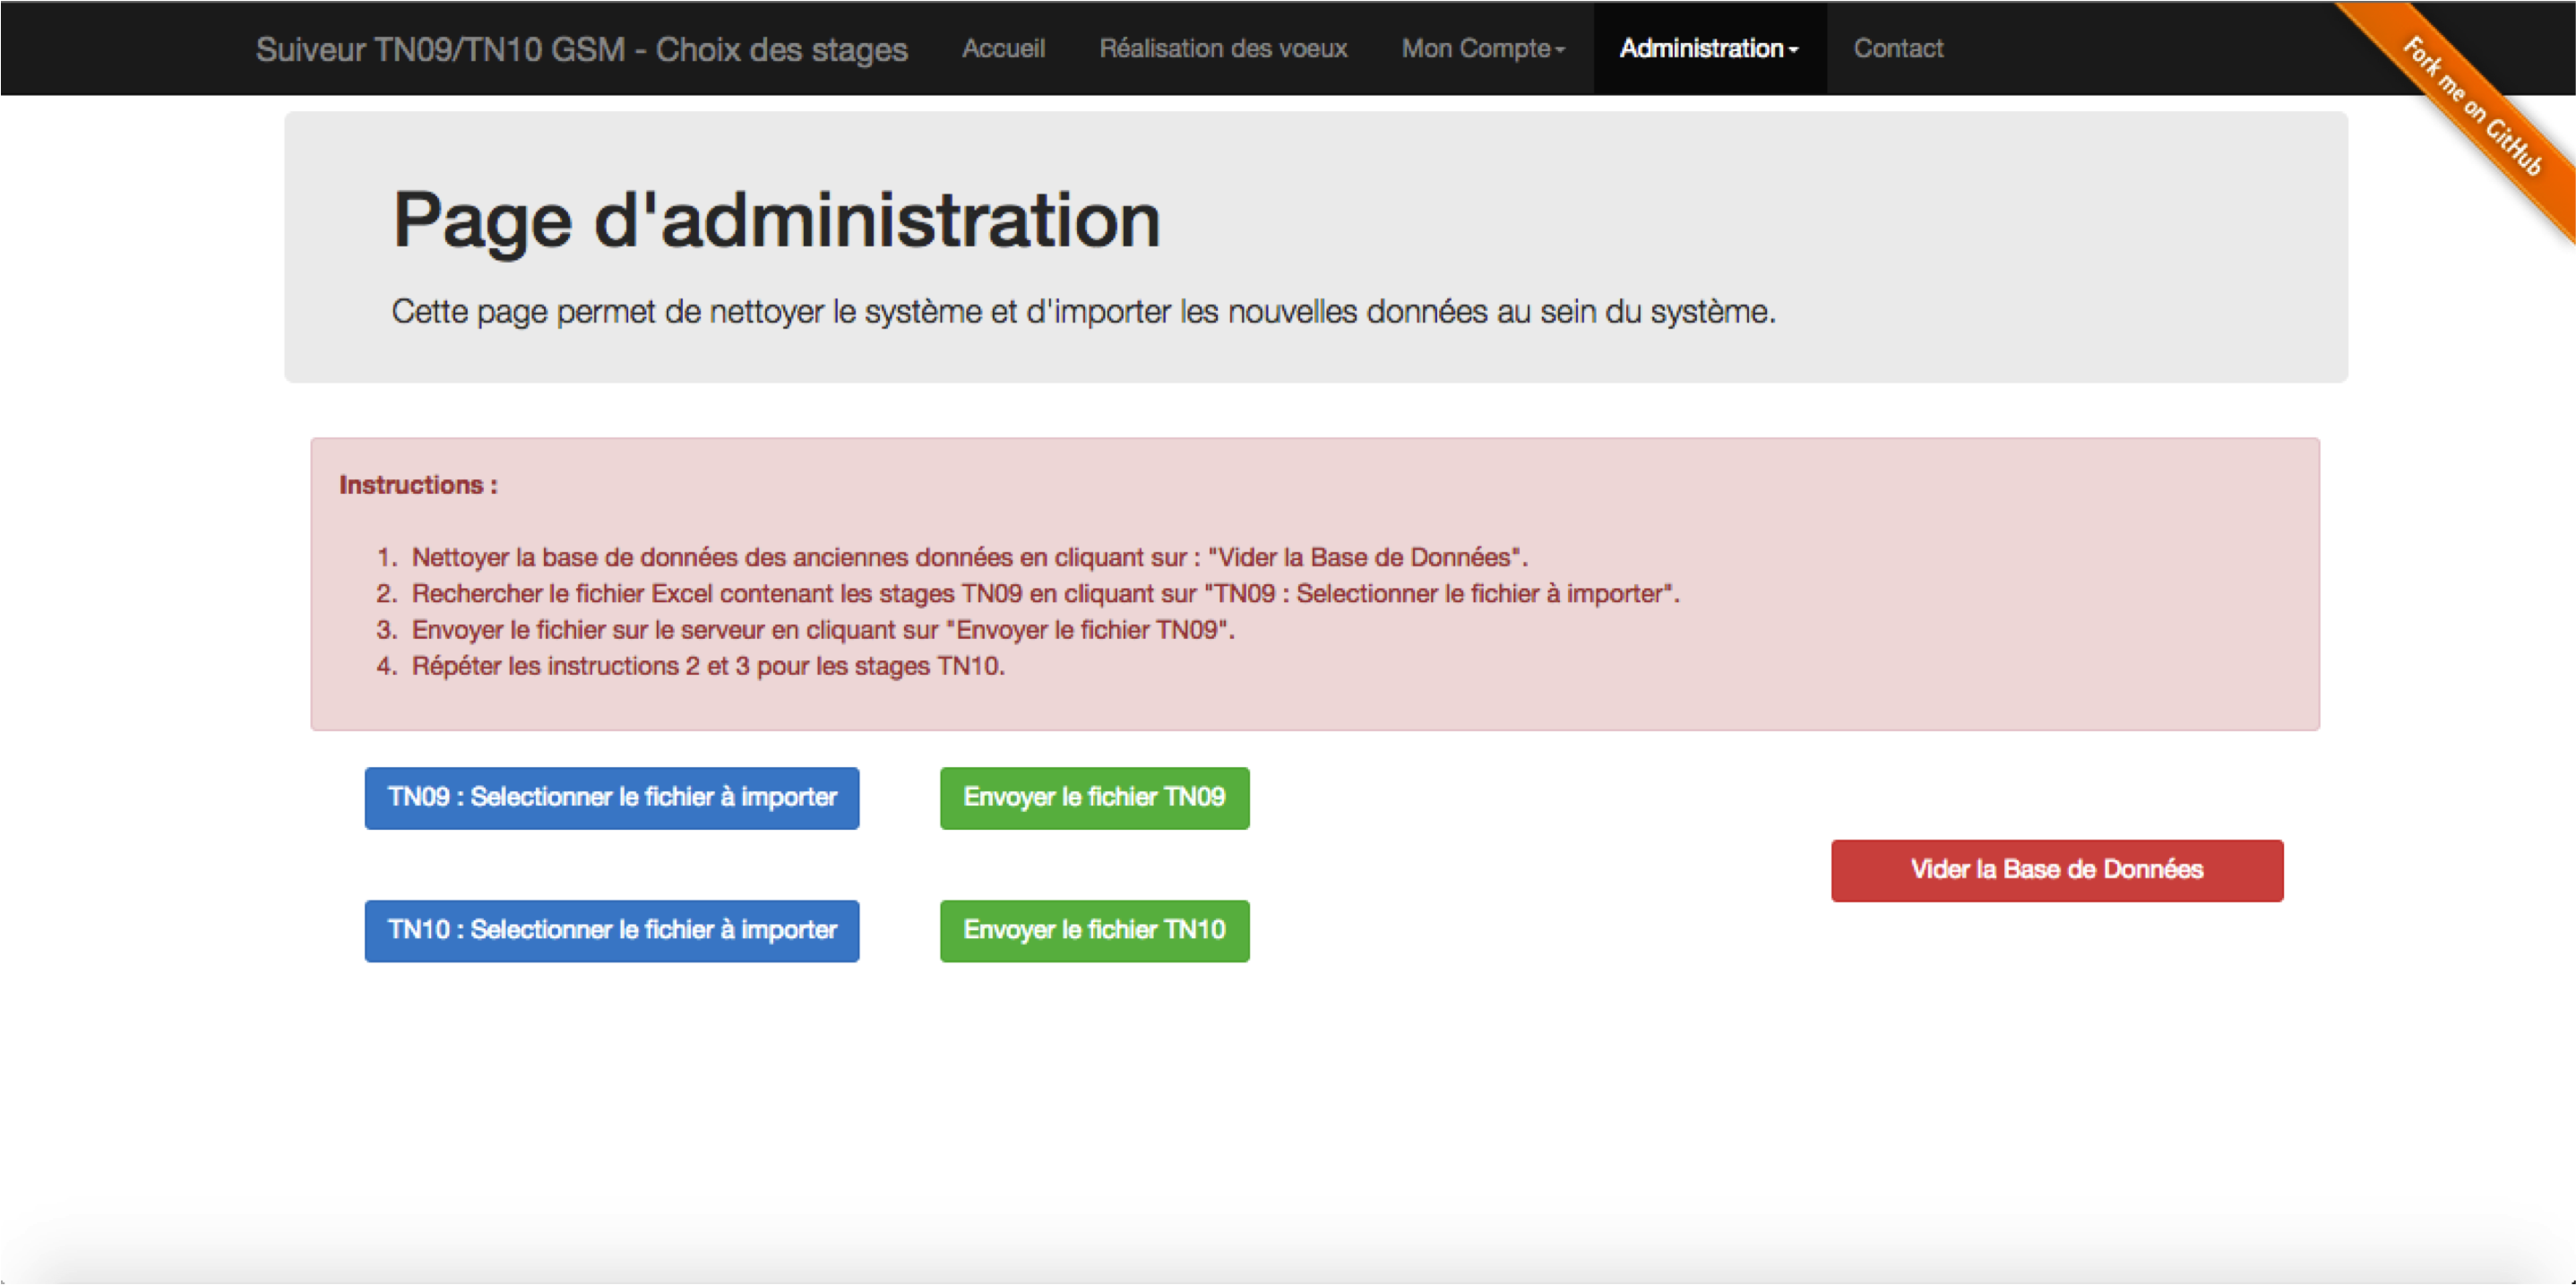
\includegraphics[scale=0.33]{Images/admin_upload.png}
		\caption{Panneau d'import des stages.}
		\vspace{-5mm}
	\end{center}
\end{figure}

\textbf{Opérations à mener pour importer les stages sur la plateforme :}

\vspace{5mm}

\begin{enumerate}
	\item Nettoyer la base de données des anciennes données en cliquant sur : \textit{"Vider la Base de Données"}.\\
	
	\item Rechercher le fichier Excel contenant les stages TN09 en cliquant sur \textit{"TN09 : Selectionner le fichier à importer"}.\\
	
	\item Envoyer le fichier sur le serveur en cliquant sur \textit{"Envoyer le fichier TN09"}.\\

	
	\item Répéter les instructions 2 et 3 pour les stages TN10.
	
\end{enumerate}

\clearpage

\LARGE
\begin{center}
\textbf{- Attention -}\\
\end{center}
\normalsize

Le fichier Excel envoyé par l'administration est légèrement corrompu, afin de le remettre d'aplomb, il faut l'ouvrir \textbf{avant l'envoie} et l'\textbf{enregistrer sous} par dessus. Cette opération remettra à plat le format du fichier. Cette opération est à réaliser pour \textbf{chacun des fichiers Excel avant l'import}.

\subsection{Export des stages au format Excel}

\begin{figure}[H]
	\vspace{-3mm}
	\begin{center}
		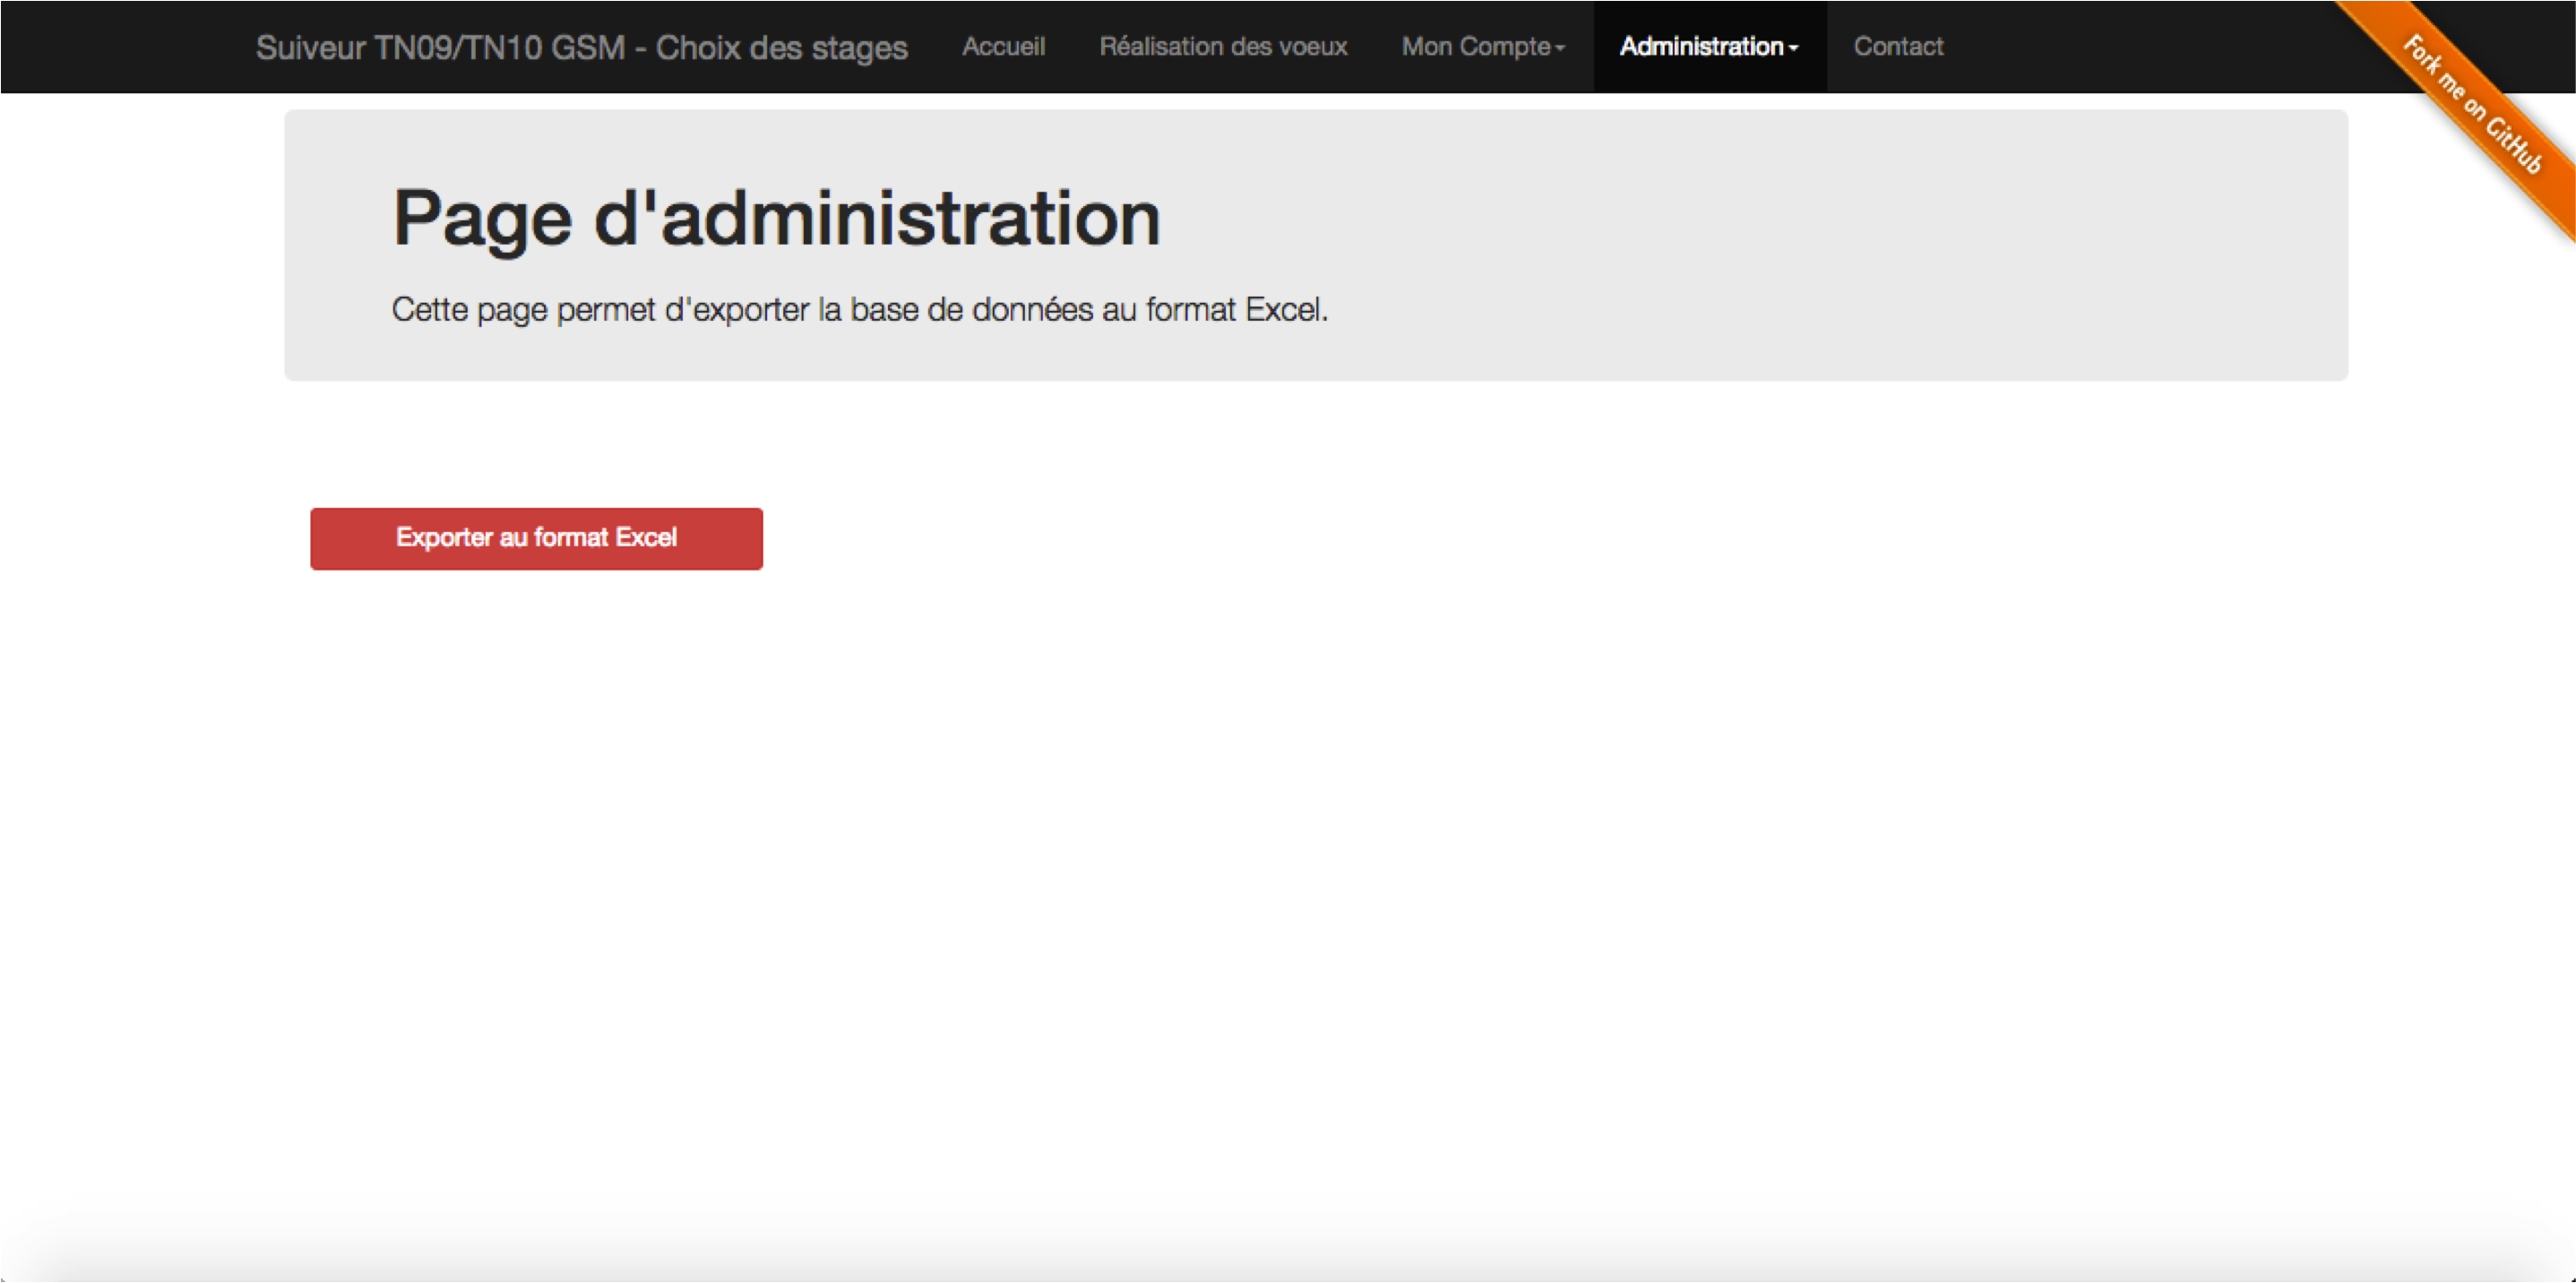
\includegraphics[scale=0.33]{Images/admin_export.png}
		\caption{Panneau d'export des stages au format Excel.}
		\vspace{-5mm}
	\end{center}
\end{figure}


Le format d'export a été défini par M. Durupt, pour le générer il suffit de cliquer sur le bouton \textit{"Exporter au format Excel"}.\\

\begin{figure}[H]
	\vspace{-3mm}
	\begin{center}
		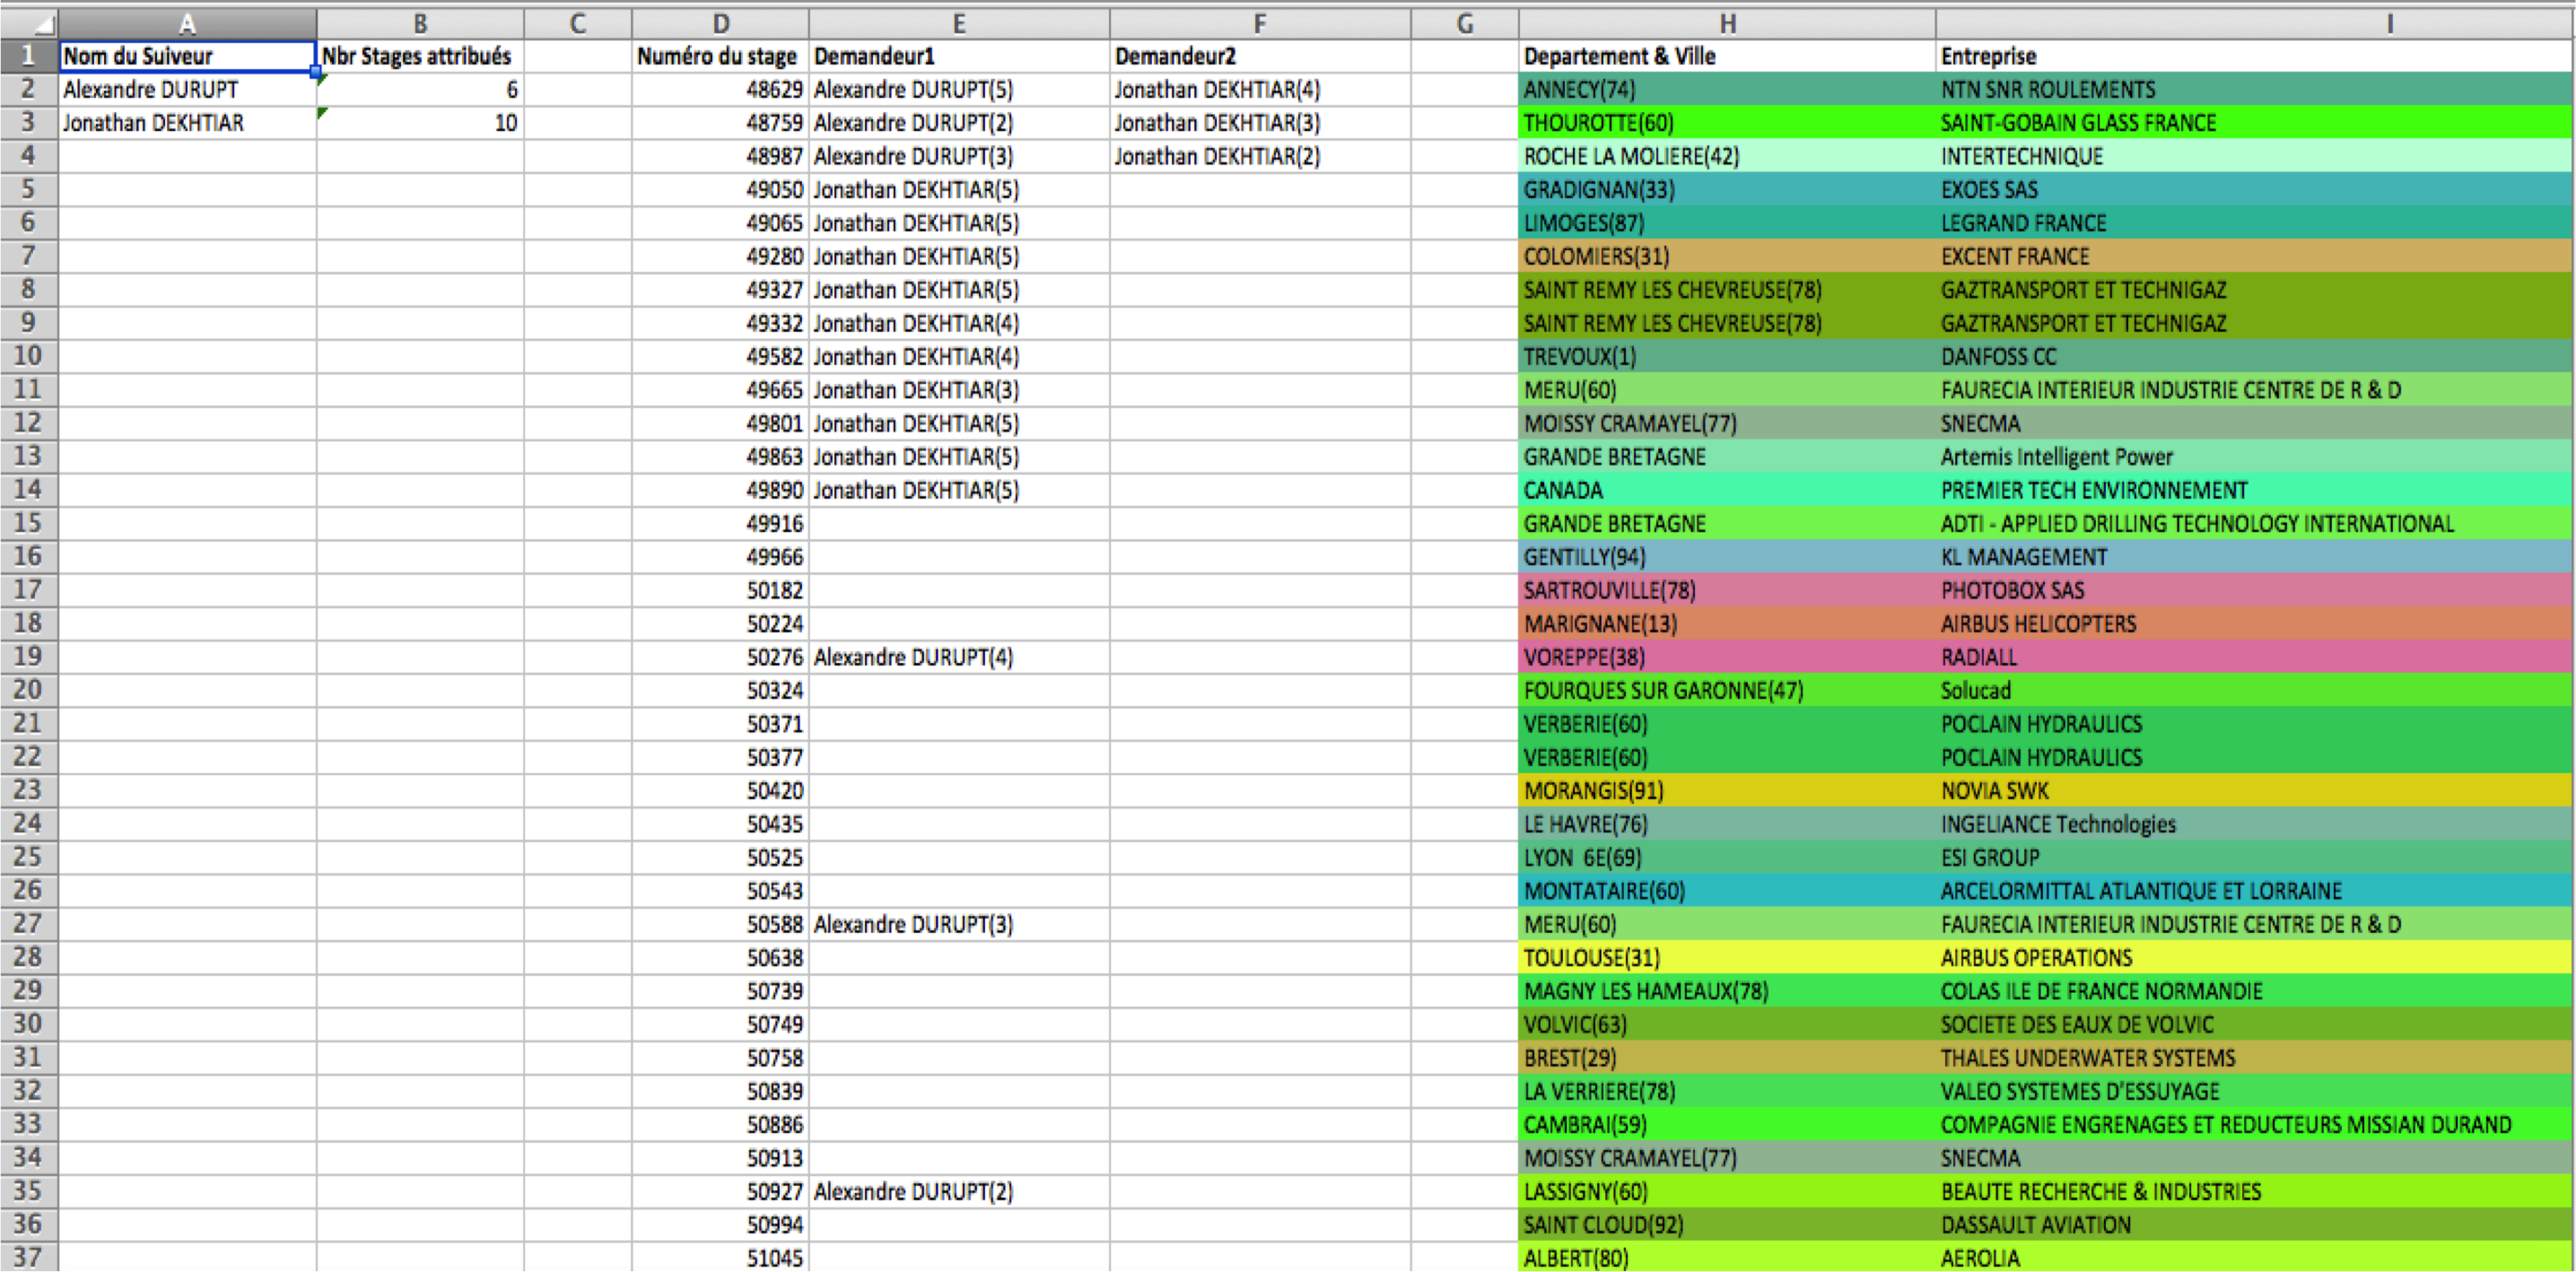
\includegraphics[scale=0.33]{Images/admin_excel.png}
		\caption{Panneau d'export des stages au format Excel.}
		\vspace{-1.5cm}
	\end{center}
\end{figure}

\clearpage

\subsection{Le Dashboard des Votes en cours}

\begin{figure}[H]
	\vspace{-3mm}
	\begin{center}
		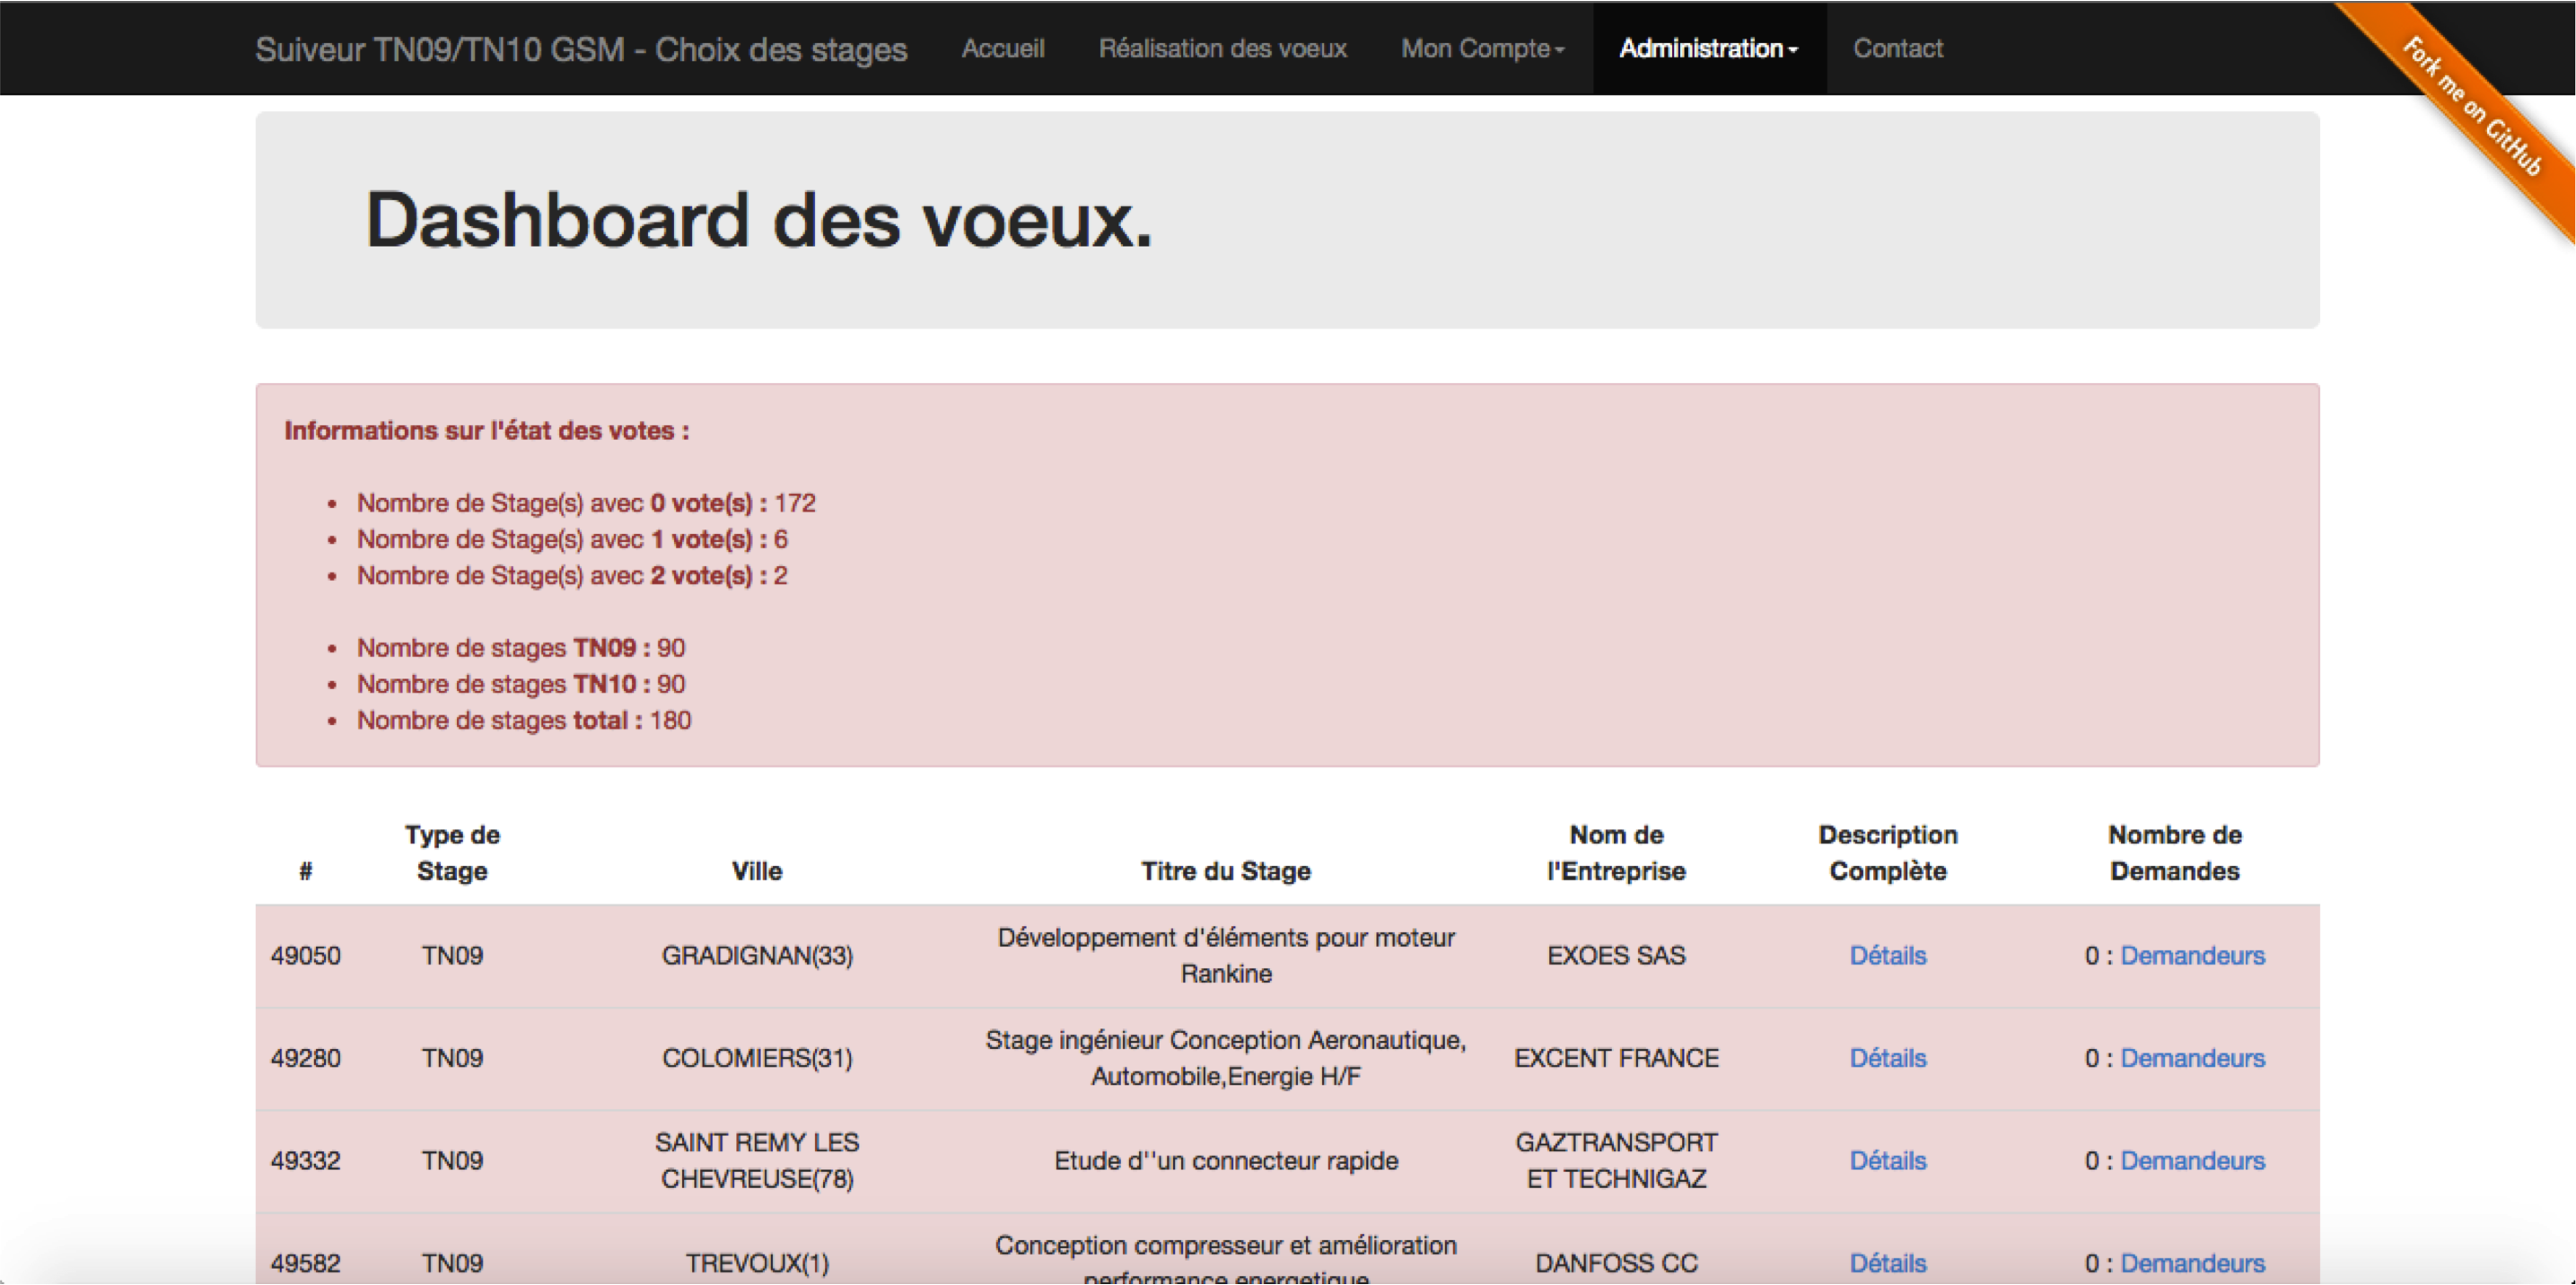
\includegraphics[scale=0.33]{Images/admin_dash1.png}
		\caption{Le Dashboard des Votes en cours}
	\end{center}
\end{figure}

\begin{figure}[H]
	\vspace{-3mm}
	\begin{center}
		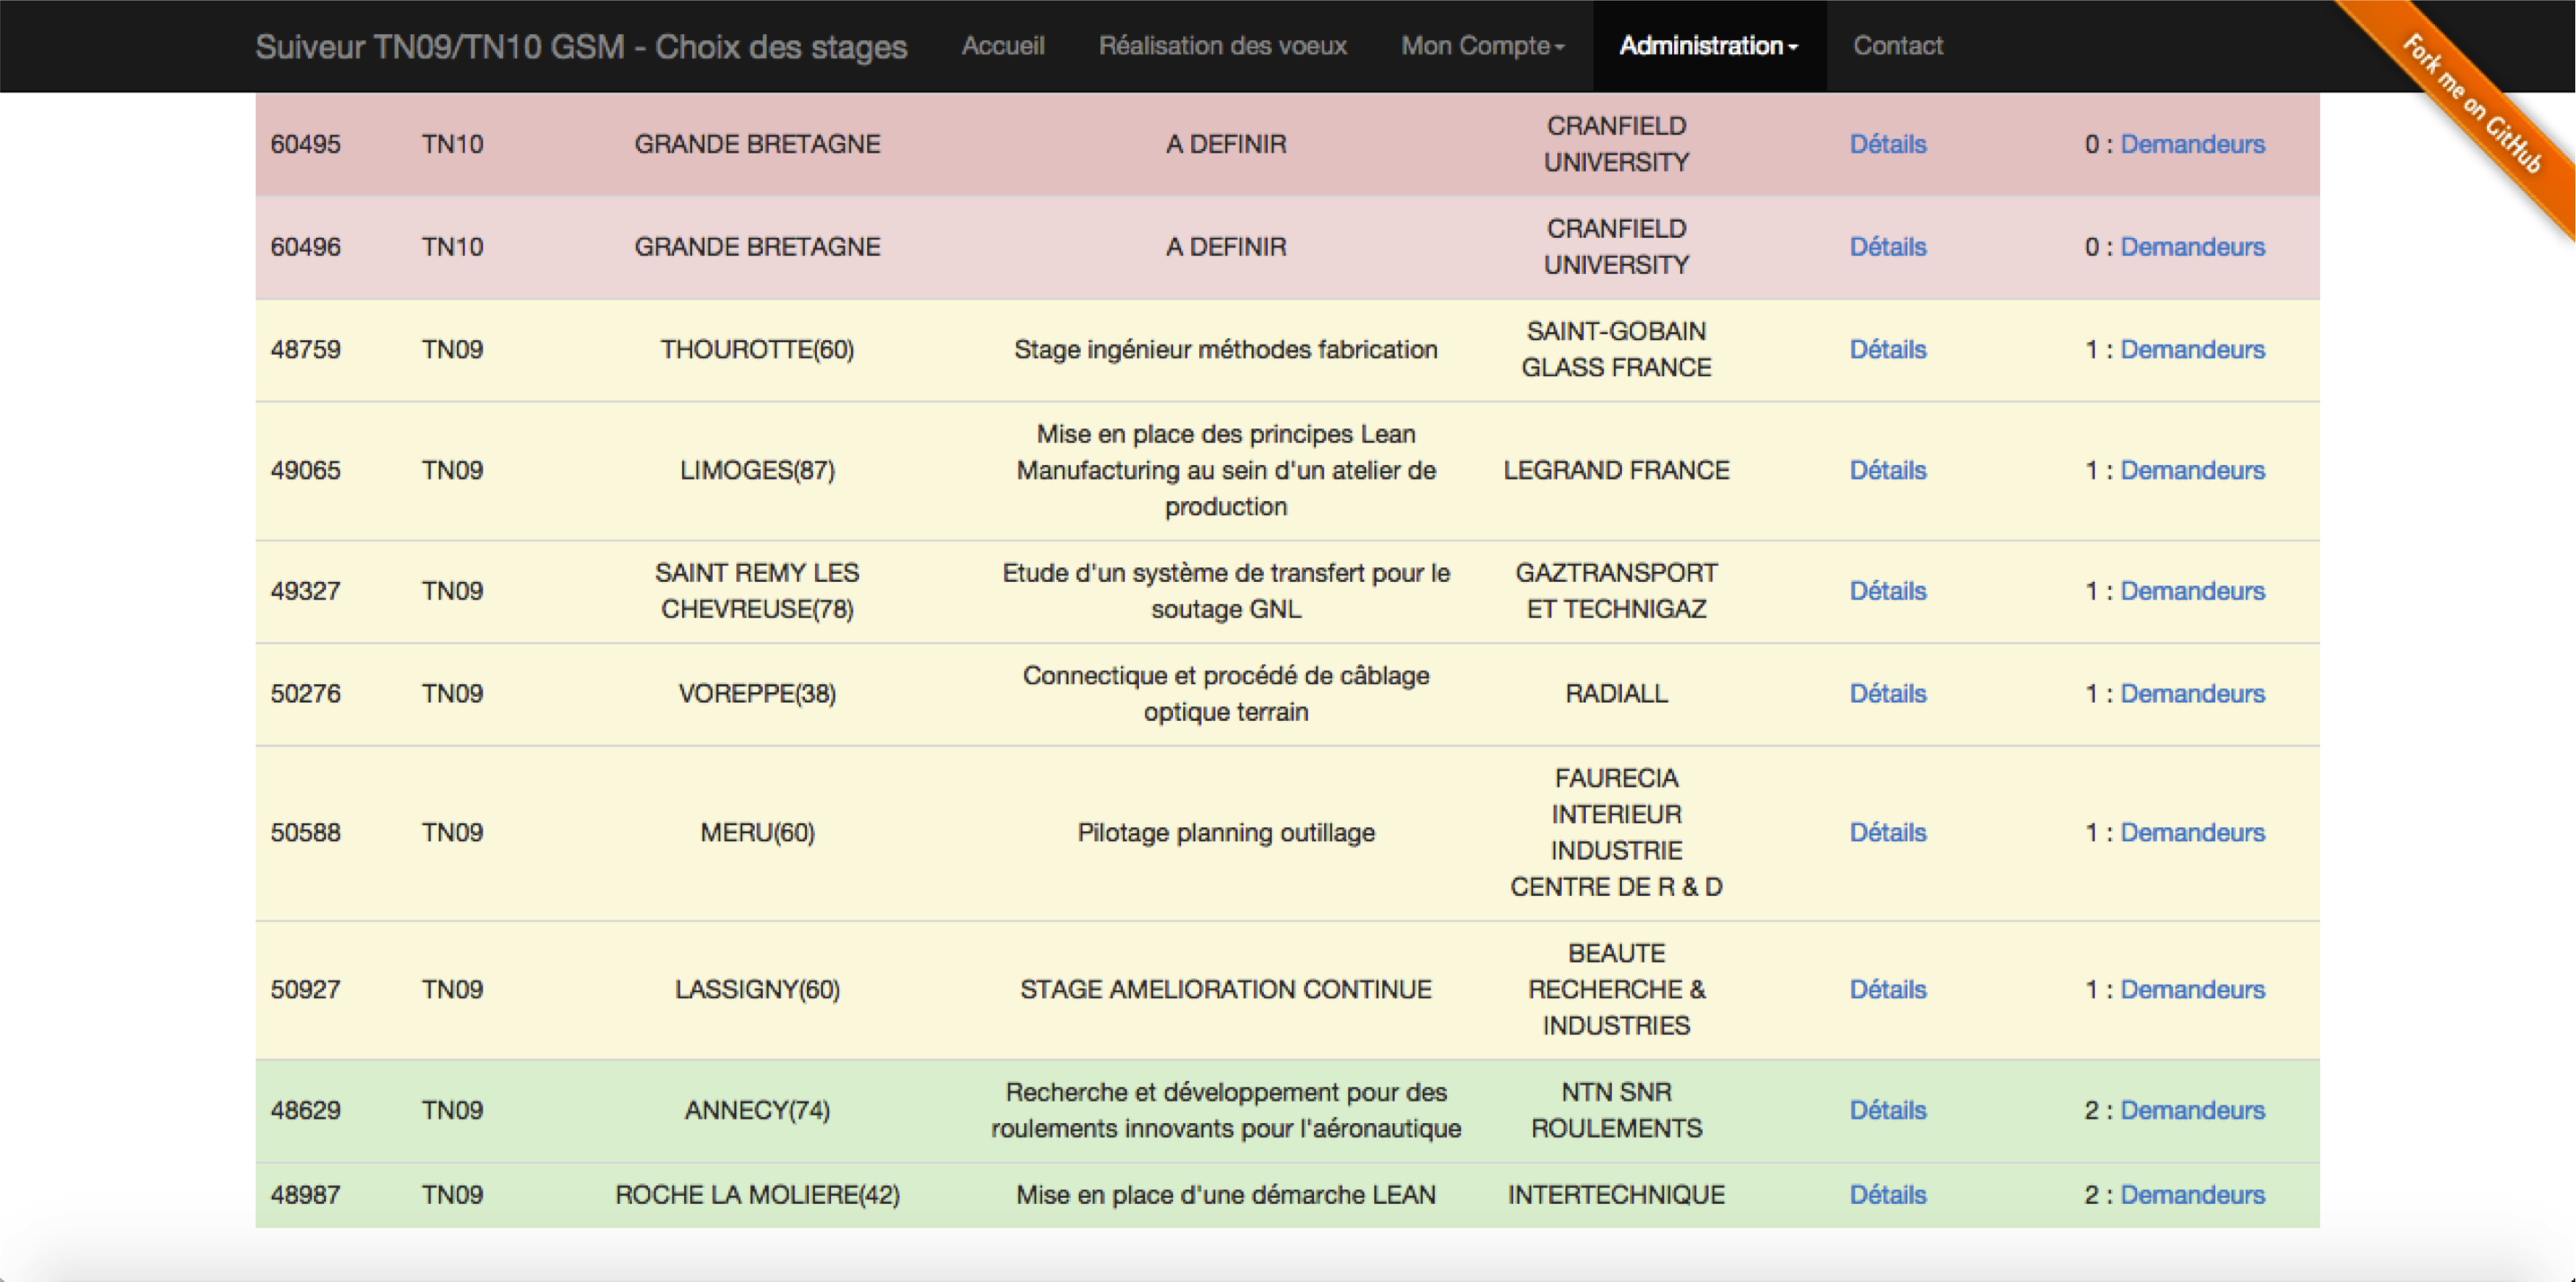
\includegraphics[scale=0.33]{Images/admin_dash2.png}
		\caption{Le Dashboard des Votes en cours}
	\end{center}
\end{figure}

Le Dashboard des Votes en cours permet de voir quels sont les stages qui n'ont pas eu de preneur, dans l'optique de leur faire "un peu de pub", ces stages apparaissent en premier dans la liste et leur couleur est \textbf{rouge}.\\

On retrouve donc plus bas les stages ayant un vote ou plus, ceux en \textbf{jaune} n'ont reçu qu'un vote, à partir de 2 votes, le stage passe au vert.\\

Il est possible d'afficher les \textbf{détails du stage} de manière identique à la page de vote et également de faire apparaitre les demandeurs pour chacun des stages en cliquant sur \textit{"Demandeurs"}.\\


\begin{figure}[H]
	\vspace{-3mm}
	\begin{center}
		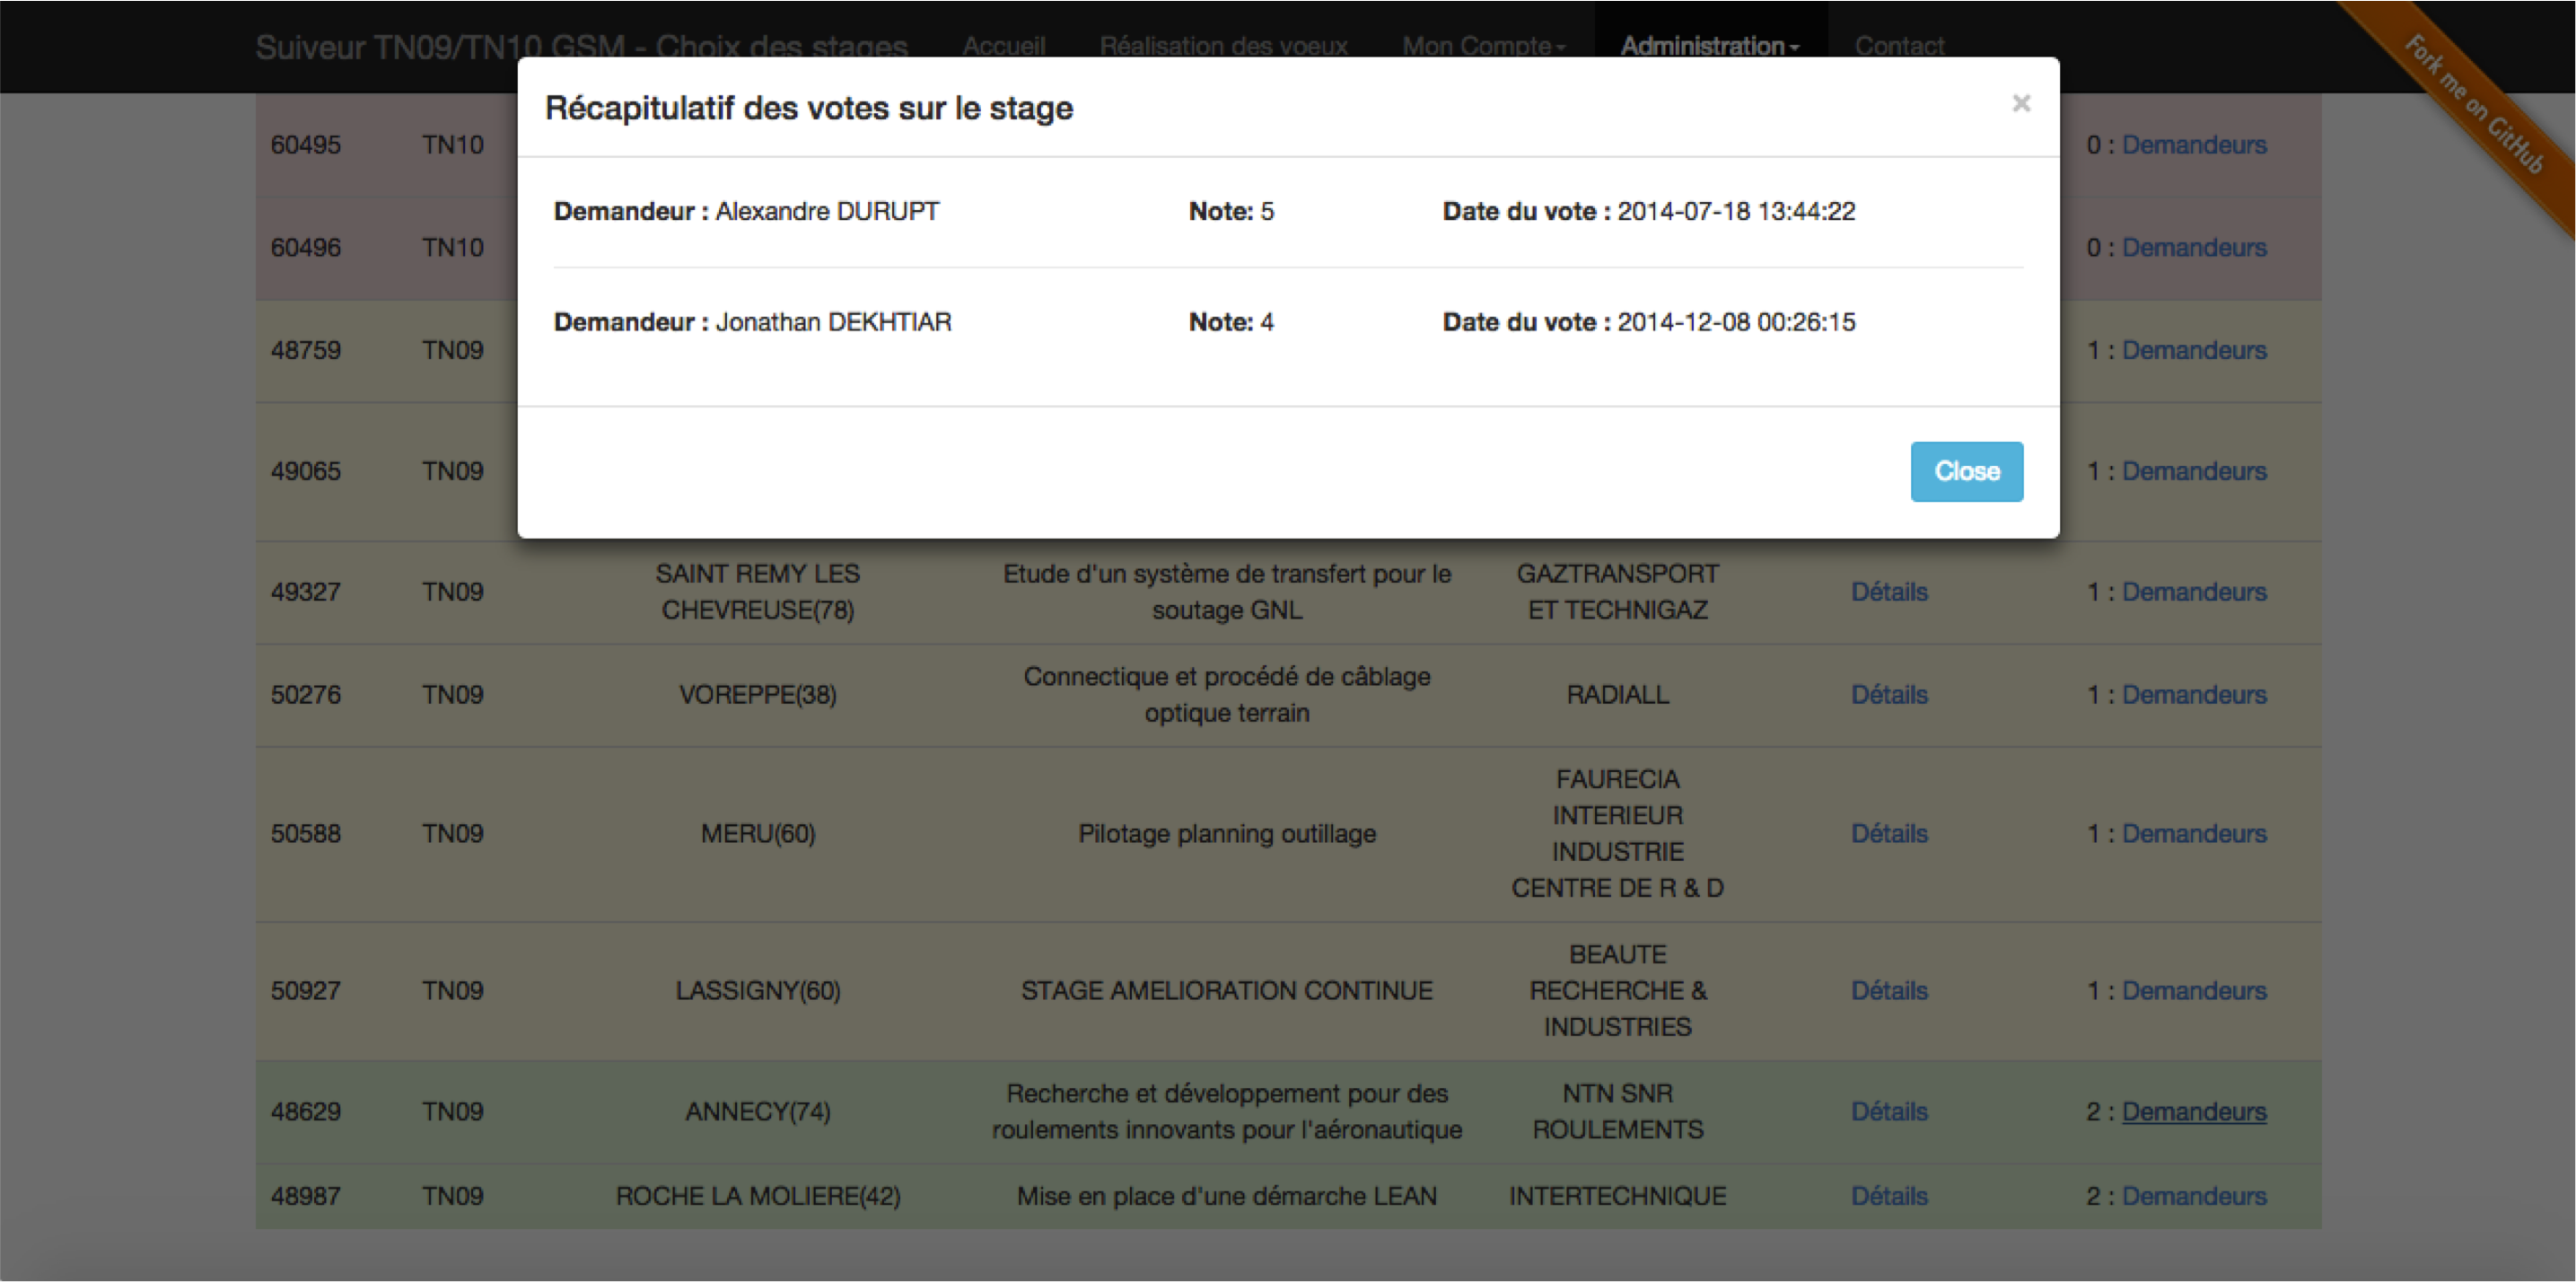
\includegraphics[scale=0.33]{Images/admin_voters.png}
		\caption{Les demandeurs pour un stage précis}
		\vspace{-5mm}
	\end{center}
\end{figure}

\clearpage
%------------------------------------------------------------------------------

\section{Pour aller plus loin ...}

\subsection{Les avantages du système}

\begin{figure}[H]
	\vspace{-3mm}
	\begin{center}
		
\includegraphics[scale=0.33]{Images/avantages.png}
		\caption{Les avantages du système}
	\end{center}
\end{figure}

\subsection{Quel futur pour le projet ?}

\begin{figure}[H]
	\vspace{-3mm}
	\begin{center}
		
\includegraphics[scale=0.33]{Images/futur.png}
		\caption{Quels possibles futurs ?}
		\vspace{-1.5cm}
	\end{center}
\end{figure}

\clearpage

%------------------------------------------------------------------------------

\section{Pour un complément d'informations}

\begin{figure}[H]
	\vspace{-3mm}
	\begin{center}
		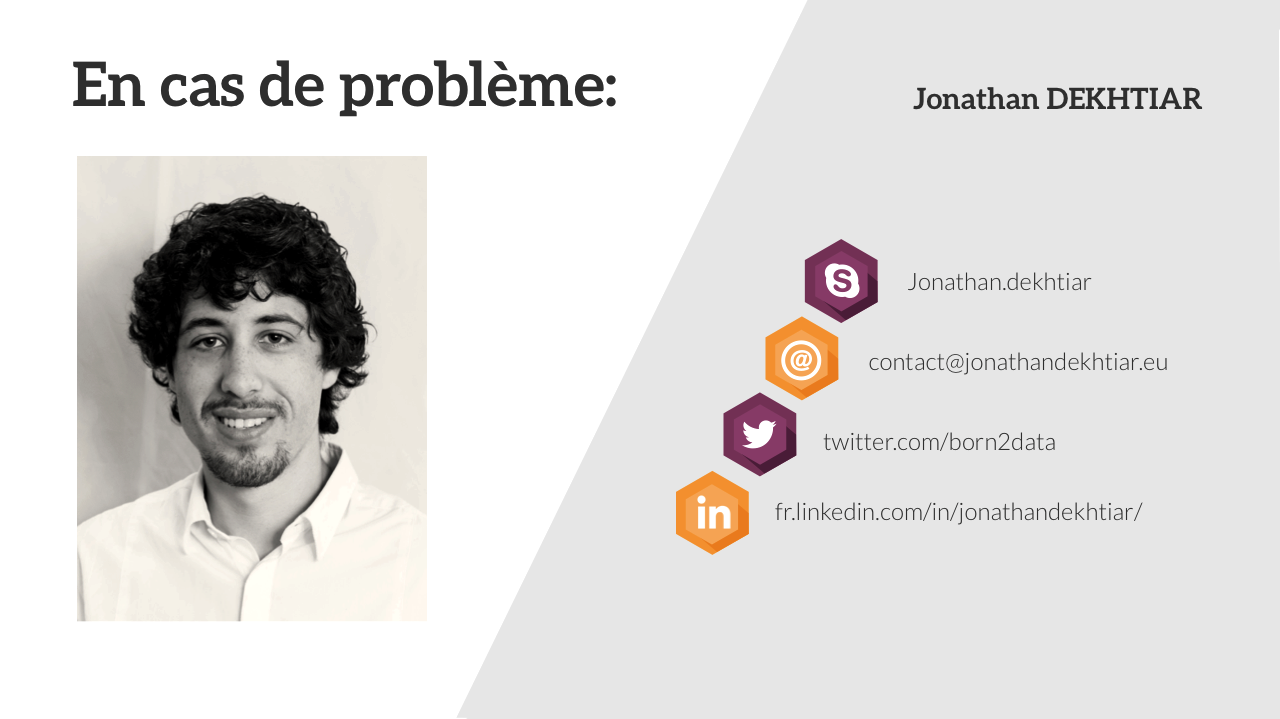
\includegraphics[scale=0.33]{Images/john.png}
		\caption{Me contacter}
	\end{center}
\end{figure}

\Large

\begin{center}
\textbf{Une documentation technique sera fourni en complément de la documentation utilisateur / administrateur.}
\end{center}

\end{document}